% LaTeX source for ``Think Bayes: Bayesian Statistics Made Simple''
% Copyright 2012  Allen B. Downey.

% License: Creative Commons Attribution-NonCommercial 3.0 Unported License.
% http://creativecommons.org/licenses/by-nc/3.0/
%

\documentclass[12pt]{book}
\usepackage[width=5.5in,height=8.5in,
  hmarginratio=3:2,vmarginratio=1:1]{geometry}

% for some of these packages, you might have to install
% texlive-latex-extra (in Ubuntu)

\usepackage[T1]{fontenc}
\usepackage{textcomp}
\usepackage{mathpazo}
\usepackage{url}
\usepackage{graphicx}
\usepackage{subfig}
\usepackage{amsmath}
\usepackage{amsthm}
\usepackage{makeidx}
\usepackage{setspace}
\usepackage{hevea}                           
\usepackage{upquote}
\usepackage{fancyhdr}

\title{Think Bayes}
\author{Allen B. Downey}

\newcommand{\thetitle}{Think Bayes: Bayesian Statistics Made Simple}
\newcommand{\theversion}{0.11.0}

% these styles get translated in CSS for the HTML version
\newstyle{a:link}{color:black;}
\newstyle{p+p}{margin-top:1em;margin-bottom:1em}
\newstyle{img}{border:0px}

% change the arrows in the HTML version
\setlinkstext
  {\imgsrc[ALT="Previous"]{back.png}}
  {\imgsrc[ALT="Up"]{up.png}}
  {\imgsrc[ALT="Next"]{next.png}} 

\makeindex

\newif\ifplastex
\plastexfalse

\begin{document}

\frontmatter

\ifplastex

\else
\fi

\newcommand{\PMF}{\mathrm{PMF}}
\newcommand{\PDF}{\mathrm{PDF}}
\newcommand{\CDF}{\mathrm{CDF}}
\newcommand{\ICDF}{\mathrm{ICDF}}

\ifplastex
    \usepackage{localdef}
    \maketitle

\else

\input{latexonly}

\begin{latexonly}

\renewcommand{\blankpage}{\thispagestyle{empty} \quad \newpage}

% TITLE PAGES FOR LATEX VERSION

%-half title--------------------------------------------------
\thispagestyle{empty}

\begin{flushright}
\vspace*{2.0in}

\begin{spacing}{3}
{\huge Think Bayes}\\
{\Large Bayesian Statistics Made Simple}
\end{spacing}

\vspace{0.25in}

Version \theversion

\vfill

\end{flushright}

%--verso------------------------------------------------------

\blankpage
\blankpage

%--title page--------------------------------------------------
\pagebreak
\thispagestyle{empty}

\begin{flushright}
\vspace*{2.0in}

\begin{spacing}{3}
{\huge Think Bayes}\\
{\Large Bayesian Statistics Made Simple}
\end{spacing}

\vspace{0.25in}

Version \theversion

\vspace{1in}


{\Large
Allen B. Downey\\
}


\vspace{0.5in}

{\Large Green Tea Press}

{\small Needham, Massachusetts}

\vfill

\end{flushright}


%--copyright--------------------------------------------------
\pagebreak
\thispagestyle{empty}

Copyright \copyright ~2012 Allen B. Downey.


\vspace{0.2in}

\begin{flushleft}
Green Tea Press       \\
9 Washburn Ave \\
Needham MA 02492
\end{flushleft}

Permission is granted to copy, distribute, and/or modify this document
under the terms of the Creative Commons Attribution-NonCommercial 3.0 Unported
License, which is available at \url{http://creativecommons.org/licenses/by-nc/3.0/}.

\vspace{0.2in}

\end{latexonly}


% HTMLONLY

\begin{htmlonly}

% TITLE PAGE FOR HTML VERSION

{\Large \thetitle}

{\large Allen B. Downey}

Version \theversion

\vspace{0.25in}

Copyright 2012 Allen B. Downey

\vspace{0.25in}

Permission is granted to copy, distribute, and/or modify this document
under the terms of the Creative Commons Attribution-NonCommercial 3.0
Unported License, which is available at
\url{http://creativecommons.org/licenses/by-nc/3.0/}.

\setcounter{chapter}{-1}

\end{htmlonly}

\fi
% END OF THE PART WE SKIP FOR PLASTEX

\chapter{Preface}
\label{preface}

\section*{}

This version of the book is a rough draft.  I am making this draft
available for comments, but it comes with the warning that it is
probably full of errors.

If you find some of those errors, please let me know.  But it is
probably too early to bother with typos.

\subsection*{Who is this book for?}

The premise of this book is that if you know how to program, you
can use that skill to help you learn other topics, including
Bayesian statistics.

Most books on Bayesian statistics use mathematical notation, and
present ideas in terms of mathematical concepts like calculus.
This book uses Python code instead of math, and discrete approximations
instead of continuous mathematics.  As a result, what would
be an integral in a math book becomes a simple summation, and
most operations on distributions are simple loops.

This presentation is easier to understand, at least for people with
programming skills.  It is also more general, because when we make
modeling decisions, we can choose the most appropriate model without
excessive concern about whether the model lends itself to conventional
analysis.

And while it's true that the discrete computations I present here
yield approximations of the results we would get from continuous
functions, it is important to remember that both computations are
based on models of a real system, and that any approximation errors
(differences between the models) are almost always negligible compared
to modeling errors (differences between the models and reality).

If, as is often the case, the discrete approach allows us to make
better modeling decisions, then it would be more fair to say that
the continuous functions yield an approximation of the
more reliable computational results.

However, I have to acknowledge that continuous analysis often yields
substantial performance advantages, for example by replacing a
linear- or quadratic-time computation with a constant-time
solution.

Therefore, I recommend a general approach with these steps:

\begin{enumerate}

\item While you are exploring a problem, start with simple models
and implement them in code that is clear, readable, and demonstrably
correct.  Focus your attention on good modeling decisions, not
optimization.

\item If the performance of your solution is good enough for your
application, stop!

\item If opt

\end{enumerate}


\subsection*{Code style}

Experienced Python programmers will notice that the code in this
book does not comply with PEP 8, which is the most common
style guide for Python (\url{http://www.python.org/dev/peps/pep-0008/}).

In particular, PEP 8 calls for lowercase function names with
underscores between words, \verb"like_this".  In this book and
the accompanying code, function and method names begin with
a capital letter and use camel case, \verb"LikeThis".

The reason I broke this rule is that I developed some of the
code while I was a Visiting Scientist at Google, Inc. in 2009-10.
So I followed the Google style guide for Python, which deviates
from PEP 8 in a few places.

Also, once I got used to function names with capital letters, I
found that I liked it.  Finally, at this point, it would be too
much trouble to change.


Allen B. Downey \\*
Needham MA \\*

Allen B. Downey is a Professor of Computer Science at 
the Franklin W. Olin College of Engineering.




%\section*{Acknowledgements}



\section*{Contributor List}

If you have a suggestion or correction, please send email to 
{\tt downey@allendowney.com}.  If I make a change based on your
feedback, I will add you to the contributor list
(unless you ask to be omitted).
\index{contributors}

If you include at least part of the sentence the
error appears in, that makes it easy for me to search.  Page and
section numbers are fine, too, but not quite as easy to work with.
Thanks!

\small

\begin{itemize}

\item First, I have to acknowledge David MacKay's excellent book,
  {\it Information Theory, Inference, and Learning Algorithms} which is
  where I first came to understand Bayesian methods.  With his
  permission (and with acknowledgement) I use several problems from
  his book as examples.

\item This book has also benefited from my interactions with Sanjoy
  Mahajan, especially in Fall 2012, when I audited his class on
  Bayesian Inference at Olin College.

\item Jonathan Edwards sent in the first typo.

\item George Purkins found a markup error.

\item Olivier Yiptong send several helpful suggestions.

\item Yuriy Pasichnyk found several errors.

% ENDCONTRIB

\end{itemize}

\normalsize

\clearemptydoublepage

% TABLE OF CONTENTS
\begin{latexonly}

\tableofcontents

\clearemptydoublepage

\end{latexonly}

% START THE BOOK
\mainmatter

\newcommand{\p}[1]{\ensuremath{\mathrm{p}(#1)}}
\renewcommand{\o}[1]{\ensuremath{\mathrm{o}(#1)}}
\newcommand{\T}[1]{\mbox{#1}}
\newcommand{\AND}{~\mathrm{and}~}
\newcommand{\NOT}{\mathrm{not}~}


\chapter{Bayes's Theorem}
\label{intro}

\section{Conditional probability}

The fundamental idea behind all Bayesian statistics is Bayes's Theorem,
which is surprisingly easy to derive, provided that you understand
conditional probability.  So we'll start with probability, then
conditional probabilty, then Bayes's Theorem, and on to Bayesian
statistics.

A probability is a number between 0 and 1 (including both) that
represents a degree of belief in a fact or prediction.  A probability
of 1 represents certainty that a fact is true, or that a prediction
will come true.  A probability of 0 represents equal certainty
that the fact is false.

Intermediate values represent degrees of certainty.  The value 0.5,
often represented as 50\%, means that a predicted outcome is
as likely to happen as not.  For example, the probability that a tossed
coin lands face up is very close to 50\%.

A conditional probability is a probability based on some background
information.  For example, I might be interested in the probability
that I will have a heart attack in the next year.  According to the
CDC, ``Every year about 785,000 Americans have a first coronary attack.
(\url{http://www.cdc.gov/heartdisease/facts.htm})''

The U.S. population is about 311 million, so the probability that a
randomly-chosen American will have a heart attack in the next year is
roughly 0.3\%.

But I am not a randomly-chosen American.  Epidemiologists have
identified many factors affect the risk of heart attacks; depending on
those factors, my risk might be higher or lower than average.

I am male, 45 years old, and I have
borderline high cholesterol.  Those factors increase my chances.
However, I have low blood pressure and I don't smoke, and
those factors decrease my chances.

Plugging everything into the online calculator at
\url{http://hp2010.nhlbihin.net/atpiii/calculator.asp}, I find that my
risk of a heart attack in the next year is about 0.2\%, slightly
less than the national average.
That value is a conditional probability, because it is based on
a number of factors that make up my ``condition.''

The usual notation for conditional probability is \p{A|B}, which
is the probability of $A$ given that $B$ is true.  In this
example, $A$ represents the prediction that I will have a heart
attack in the next year, and $B$ is the set of conditions I listed.


\section{Conjoint probability}

``Conjoint probability'' is a fancy way to say the probability that
two things are true.  I will write \p{A \AND B} to mean the
probability that $A$ and $B$ are both true.

If you learned about probability in the context of coin tosses and
dice, you might have learned the formula
%
\[ \p{A \AND B} = \p{A}~\p{B} \quad\mbox{WARNING: not always true}\]
%
For example, if I toss two coins, and $A$ means the first coin lands
face up, and $B$ means the second coin lands face up, then $\p{A} =
\p{B} = 0.5$, and sure enough, $\p{A \AND B} = \p{A}~\p{B} = 0.25$.

But this formula only works because in this case $A$ and $B$ are
independent; that is, the second event does not depend on the first.
If you tell me the first coin is heads, that does not change \p{B}.

Here is a different example where the events are not independent.
Suppose again that $A$ means the first coin lands face up, but let's
add $C$, which means that {\em both} coins land face up.  What is the
probability of both events, \p{A \AND C}?

These events are dependent because if we know whether or not $A$ is
true, that changes \p{C}.  Specifically, if $A$ is true then $\p{C}
= 0.5$; but if $A$ is false $\p{C} = 0$.

To be more correct, I should not say that \p{C} changes, but
rather that the conditional probabilities are different: $\p{C|A} = 0.5$
and $\p{C| \NOT A} = 0$.

In general, the probability of a conjunction is
%
\[ \p{A \AND C} = \p{A}~\p{C|A} \]
%
for any $A$ and $C$.  In this example, \p{A \AND C} = (0.5)(0.5) = 0.25.


\section{The Cookie Problem}

We'll get to Bayes's Theorem soon, but I want to motivate it with an
example called The Cookie Problem\footnote{Based on an example from
  \url{http://en.wikipedia.org/wiki/Bayes'_theorem} that is no longer
  there.}.  Suppose there are two bowls of cookies.  Bowl 1 contains
  30 vanilla cookies and 10 chocolate cookies.  Bowl 2 contains 20 of
  each.

Now suppose you choose one of the bowls at random and, without looking,
select a cookie at random.  The cookie is vanilla.  What is the probability
that it came from Bowl 1?

This is a conditional probability; we want \p{\T{Bowl 1} | \T{vanilla}},
but it is not obvious how to compute it.  On the other
hand, if we flip it around, it's very easy:
%
\p{\T{vanilla} | \T{Bowl 1}} = 3/4
%
Unfortunately, \p{A|B} is {\em not} the same as \p{B|A}.  But there
is a way to get from one to the other: Bayes's Theorem.


\section{Bayes's Theorem}

At this point we have everything we need to derive Bayes's Theorem.
We'll start with the observation that conjunction is commutative; that is
%
\[ \p{A \AND B} = \p{B \AND A} \]
%
for any events $A$ and $B$.

Next, we write the probability of a conjunction:
%
\[ \p{A \AND B} = \p{A}~\p{B|A} \]
%
Since we have not said anything about what $A$ and $B$ mean, they
are interchangeable.  Interchanging them yields
%
\[ \p{B \AND A} = \p{B}~\p{A|B} \]
%
And that's all we need.  Pulling those pieces together, we get
%
\[ \p{B}~\p{A|B} = \p{A}~\p{B|A} \]
%
Which means there are two ways to compute the conjunction.
If you have \p{A}, you multiply by the conditional
probability \p{B|A}.  Or you can do it the other way around; if you
know \p{B}, you multiply by \p{A|B}.  Either way you should get
the same thing.

Finally we can divide through by \p{B}
%
\[ \p{A|B} = \frac{\p{A}~\p{B|A}}{\p{B}} \]
%
And that's Bayes's Theorem!  It doesn't look like much, but
it is a surprisingly powerful idea.

For example, we can use it to solve the Cookie Problem.  I'll write
$B_1$ for the hypothesis that the cookie came from Bowl 1
and $V$ for the vanilla cookie.  Plugging in Bayes's Theorem
we get
%
\[ \p{B_1|V} = \frac{\p{B_1}~\p{V|B_1}}{\p{V}} \]
%
The term on the left is what we want: the probability of Bowl 1, given
that we chose a vanilla cookie.  The terms on the right are:

\begin{itemize}

\item \p{B_1}: This is the probability that we chose Bowl 1, unconditioned
by what kind of cookie we got.  Since the problem says we chose a
bowl at random, we can assume \p{B_1} = 1/2.

\item \p{V|B_1}: This is the probability of getting a vanilla cookie
from Bowl 1, which is 3/4.

\item \p{V}: This is the probability of drawing a vanilla cookie from
either bowl.  If we combine the two bowls, we get 50 vanilla and 30
chocolate cookies, so \p{V} = 5/8.

\end{itemize}

Putting it together, we have 
%
\[ \p{B_1|V} = \frac{(1/2)(3/4)}{5/8} \]
%
which reduces to 3/5.  So the vanilla cookie is evidence in favor of
the hypothesis that we chose Bowl 1, because vanilla cookies are more
likely to come from Bowl 1.

This example demonstrates one use of Bayes's Theorem: it provides
a process to get from \p{B|A} to \p{A|B}.  This strategy is useful
in cases, like the Cookie Problem, where it is easier to compute
the terms on the right side of Bayes's Theorem than the term on the
left.


\section{The diachronic interpretation}

There is another way to think of Bayes's Theorem: it gives us a
way to update the probability of a hypothesis, $H$, in light of
some body of data, $D$.

This way of thinking about Bayes's Theorem is called the
{\bf diachronic interpretation}.  ``Diachronic'' means that something
is happening over time; in this case there is an implicit notion
that the probability of the hypotheses changes, over time, as
we see new data.

Rewriting Bayes's Theorem with $H$ and $D$ yields:
%
\[ \p{H|D} = \frac{\p{H}~\p{D|H}}{\p{D}} \]
%
In this interpretation, each term has a name:

\begin{itemize}

\item \p{H} is the probability of the hypothesis before we see
the data, called the prior probability, or just {\bf prior}.

\item \p{H|D} is what we want to compute, the probability of
the hypothesis after we see the data, called the {\bf posterior}.
 
\item \p{D|H} is the probability of the data under the hypothesis,
called the {\bf likelihood}.

\item \p{D} is the probability of the data under any hypothesis,
called the {\bf normalizing constant}.

\end{itemize}

In some cases, we can compute the prior
based on background information.  For example, the Cookie
Problem specifies that we choose a bowl at random (and implies
that they have equal probability).

In other cases the prior
is subjective; that is, reasonable people might disagree,
either because they use different background information
or because they interpret the same information differently.

The likelihood is usually the easiest part to compute.  In the
Cookie Problem, if we know which bowl the cookie came from,
we can get the probability of getting a vanilla cookie by counting.

The normalizing constant can be tricky.  It is supposed to be the
probability of seeing the data under any hypothesis at all, but in the
most general case it is hard to see what that means.

Most often we simplify things by specifying a set of hypotheses
that are

\begin{description}

\item[Mutually exclusive:] which means that only one hypothesis in
the set can be true, and

\item[Collectively exhaustive:] which means that there are no other
possibilities; one of the hypotheses has to be true.

\end{description}

I use the word {\bf suite} for a set of hypotheses that has these
properties.

In the Cookie Problem, there are only two hypotheses---the cookie
came from Bowl 1 or Bowl 2---and they are mutually exclusive and
collectively exhaustive.

In that case we can compute \p{D} using the law of total probability,
which says that if there are two exclusive ways that something
might happen, you can add up the probabilities like this:
%
\[ \p{D} = \p{B_1}~\p{D|B_1} + \p{B_2}~\p{D|B_2} \]
%
Plugging in the values from the Cookie Problem, we have
%
\[ \p{D} = (1/2)~(3/4) + (1/2)~(1/2) = 5/8 \]
%
which is what we computed earlier by mentally combining the two
bowls.


\newcommand{\MM}{M\&M}

\section{The \MM~Problem}

\MM's are small candy-coated chocolates that come in a variety of
colors.  Mars, Inc., which makes \MM's, changes the mixture of
colors from time to time.

In 1995, they introduced blue \MM's.  Before then, the color mix in
a bag of plain M\&Ms was (30\% Brown, 20\% Yellow, 20\% Red, 10\%
Green, 10\% Orange, 10\% Tan).  Afterward it was (24\% Blue , 20\%
Green, 16\% Orange, 14\% Yellow, 13\% Red, 13\% Brown).

%\index{M\&M}

A friend of mine has two bags of \MM's, and he tells me
that one is from 1994 and one from 1996.  He won't tell me which is
which, but he gives me one \MM~from each bag.  One is yellow and
one is green.  What is the probability that the yellow one came
from the 1994 bag?

This problem is similar to the Cookie Problem, with the twist that I
draw one sample from each bowl/bag.  This problem also gives me a
chance to demonstrate the table method, which is useful for solving
problems like this on paper.  In the next chapter we will
solve them computationally.

The first step is to enumerate the hypotheses.  In this case there
are only two:

\begin{itemize}

\item A: the yellow \MM~is from 1994, which implies that green is
from 1996.

\item B: the yellow \MM~is from 1996 and green from 1994.

\end{itemize}

Now we construct a table with a row for each hypothesis and a
column for each term in Bayes's Theorem:

\begin{tabular}{|c|c|c|c|c|}
\hline
   & \p{H} & \p{D|H} & \p{H}~\p{D|H}  & \p{H|D}  \\
\hline
A  &  1/2  &  (20)(20)  &  200  &  20/27 \\
B  &  1/2  &  (10)(14)  &   70  &  7/27 \\
\hline
\end{tabular}

The first column has the priors.
Since there is one bag from 1994 and one from 1996,
it is reasonable to choose $\p{A} = \p{B} = 1/2$.

The second column has the likelihoods, which follow from the
information in the problem.  If $A$ is true, the yellow \MM~came from
1994 with probability 20\%, and the green came from 1996 with
probability 20\%.  Because the selections are
independent, we get the conjoint probability by multiplying.

The third column is just the product of the previous two.
The sum of this column, 270, is the normalizing constant.
To get the last column, which contains the posteriors, we divide
the third column by the normalizing constant.

That's it.  Simple, right?

Well, you might be bothered by one detail.  I wrote \p{D|H}
in terms of percentages, not probabilities, which means it
is off by a factor of 10,000.  But that
cancels out when we divide through by the normalizing factor, so
it doesn't affect the result.

When the set of hypotheses is mutually exclusive and collectively
exhaustive, you can multiply the likelihoods by any factor,
if it is convenient, as long as you apply the same factor to the entire
column.


\section{The Monty Hall problem}

The Monty Hall problem might be the most contentious question in
the history of probability.  The scenario is simple, but the correct
answer is so counter-intuitive that many people just can't accept
it, and many smart people have embarrassed themselves not just by
getting it wrong but by arguing the wrong side, aggressively,
in public.

Monty Hall was the original host of the game show {\em Let's Make a
Deal}.  The Monty Hall problem is based on one of the regular
games on the show.  If you are on the show, here's what happens:

\begin{itemize}

\item Monty shows you three closed doors and tells you that there is a
  prize behind each door: one prize is a car, the other two are less
  valuable prizes like peanut butter and fake finger nails.  The
  prizes are arranged at random.

\item The object of the game is to guess which door has the car.  If
  you guess right, you get to keep the car.

\item So you pick a door, which we will call Door A.  We'll call the
  other doors B and C.

\item Before opening the door you chose, Monty increases the
  suspense by opening either Door B or C, whichever does not
  have the car.  (If the car is actually behind Door A, Monty can
  safely open B or C, so he chooses one at random).

\item Then Monty offers you the option to stick with your original
  choice or switch to the one remaining unopened door.

\end{itemize}

The question is, should you ``stick'' or ``switch'' or does it
make no difference?
\index{stick}
\index{switch}
\index{intuition}

Most people have the strong intuition that it makes no difference.
There are two doors left, they reason, so the chance that the car
is behind Door A is 50\%.

But that is wrong.  In fact, the chance of winning if you stick
with Door A is only 1/3; if you switch, your chances are 2/3.

By applying Bayes's Theorem, we can break this problem into simple
pieces, and maybe convince ourselves that the correct answer is,
in fact, correct.

To start, we should make a careful statement of the data.  In
this case $D$ consists of two parts: Monty chooses Door B,
and there is no car there.

Next we define three hypotheses: $A$, $B$ and $C$ represent the
hypothesis that the car is behind Door A, Door B or Door C.
Again, let's apply the table method:

\begin{tabular}{|c|c|c|c|c|}
\hline
   & \p{H} & \p{D|H} & \p{H}~\p{D|H}  & \p{H|D}  \\
\hline
A  &  1/3  &  1/2  &  1/6  &  1/3 \\
B  &  1/3  &  0  &   0  &  0 \\
C  &  1/3  &  1  &   1/3  &  2/3 \\
\hline
\end{tabular}

Filling in the priors is easy because we are told that the prizes
are arranged at random, which implies that the car is equally
likely to be behind any door.

Figuring out the likelihoods takes some thought, but with reasonable
care we can be confident that we have it right:

\begin{itemize}

\item If the car is actually behind A, Monty could safely open Doors
B or C.  So the probability that he chooses B is 1/2.  And since
the car is actually behind A, the probability that the car is not
behind B is 1.

\item If the car is actually behind B, Monty does not open B, so the
probability of the data we saw is 0.

\item Finally, if the car is behind Door C, Monty opens B with probability
1 and finds no car there with probability 1.

\end{itemize}

Now the hard part is over; the rest is just arithmetic.  The
sum of the third column is 1/2.  Dividing through yields
$\p{A|D} = 1/3$ and $\p{C|D} = 2/3$.  So you are better off switching.

There are many variations of the Monty Hall problem.  One of the
strengths of the Bayesian approach is that it generalizes to handle
these variations.

For example, suppose that Monty always chooses B if he can, and
only chooses C if he has to (because the car is behind B).  In
that case the revised table is:

\begin{tabular}{|c|c|c|c|c|}
\hline
   & \p{H} & \p{D|H} & \p{H}~\p{D|H}  & \p{H|D}  \\
\hline
A  &  1/3  &  1  &  1/3  &  1/2 \\
B  &  1/3  &  0  &   0   &  0 \\
C  &  1/3  &  1  &   1/3  &  1/2 \\
\hline
\end{tabular}

The only change is \p{D|A}.  If the car is behind $A$, Monty can
chose to open B or C.  But in this variation he always chooses
B, so $\p{D|A} = 1$.

As a result, the likelihoods are the same for $A$ and $C$, and the
posteriors are the same: $\p{A|D} = \p{C|D} = 1/2$.  In this case, the
fact that Monty chose B reveals no information about the location of
the car, so it doesn't matter whether the contestant sticks or
switches.

On the other hand, if he had opened $C$, we would know $\p{B|D} = 1$.


\chapter{Computational statistics}

\section{Distributions}

In statistics a {\bf distribution} is a set of values and their
corresponding probabilities.

For example, if you roll a six-sided die, the set of possible
values is the numbers 1 to 6, and the probability associated
with each value is 1/6.

As another example, you might be interested in how many times each
word appears in common English usage.  You could build a distribution
that includes each word and how many time it appears.

In Python, you could represent a distribution with a dictionary that
maps from each value to its probability.  As an alternative, I have
written a class called {\tt Pmf} that represents a distribution.  PMF
stands for ``probability mass function'' which is the more specific
mathematical term for what I am calling a distribution.

{\tt Pmf} is defined in a Python module I wrote to accompany this
book, called {\tt thinkbayes.py}.  You can download it from
\url{http://thinkbayes.com/thinkbayes.py}.  To use {\tt Pmf} you
can import it like this:

\begin{verbatim}
from thinkbayes import Pmf
\end{verbatim}

The following code builds a Pmf to represent the distribution
of outcomes for a six-sided die:

\begin{verbatim}
pmf = Pmf()
for x in [1,2,3,4,5,6]:
    pmf.Set(x, 1/6.0)
\end{verbatim}

\verb"Pmf" creates an empty Pmf object with no values.  The
\verb"Set" method sets the probability associated with each
value to $1/6$.

Here's another example that counts the number of times each word
appears in a sequence:

\begin{verbatim}
pmf = Pmf()
for word in word_list:
    pmf.Incr(word, 1)
\end{verbatim}

\verb"Incr" increases the ``probability'' associated with each
word by 1.  If a word is not already in the Pmf, it is added.

I put ``probability'' in quotes because in this example, the
probabilities are not normalized; that is, they do not add up to 1.
So they are not true probabilities.

But in this example the word counts are proportional to the probabilities.
So after we count all the words, we can compute probabilities by
dividing through by the total number of words.  {\tt Pmf} provides
a method, \verb"Normalize", that does exactly that:

\begin{verbatim}
pmf.Normalize()
\end{verbatim}

Once you have made a Pmf object, you can ask for the probability
associated with any value:

\begin{verbatim}
print pmf.Prob('the')
\end{verbatim}

And that would print the frequency of the word ``the'' as a fraction
of the words in the list.

Pmf uses a Python dictionary to store the values and their
probabilities, so the values in the Pmf can be any hashable type.
The probabilities can be any numerical type, but they are usually
floating point numbers (type \verb"float").


\section{The Cookie Problem}

In the context of Bayes's Theorem, it is natural to use a Pmf
to map from each hypothesis to its probability.  In the Cookie
Problem, the hypotheses are $B_1$ and $B_2$.  In Python, I will
represent them with strings:

\begin{verbatim}
pmf = Pmf()
pmf.Set('Bowl 1', 0.5)
pmf.Set('Bowl 2', 0.5)
\end{verbatim}

This distribution, which contains the priors for each hypothesis,
is called (wait for it) the {\bf prior distribution}.

To update the distribution based on new data (the vanilla cookie),
we multiply each prior by the corresponding likelihood.  The likelihood
of drawing a vanilla cookie from Bowl 1 is 3/4.  The likelihood
for Bowl 2 is 1/2.

\begin{verbatim}
pmf.Mult('Bowl 1', 0.75)
pmf.Mult('Bowl 2', 0.5)
\end{verbatim}

\verb"Mult" does what you would expect.  It gets the probability
for the given value and multiplies by the given factor.

After this update, the distribution is no longer normalized, but
because these hypotheses are mutually exclusion and collectively
exhaustive, we can {\bf renormalize}:

\begin{verbatim}
pmf.Normalize()
\end{verbatim}

The result is a distribution that contains the posterior probability
for each hypothesis, which is called (wait now) the
{\bf posterior distribution}.

Finally, we can get the posterior for Bowl 1.

\begin{verbatim}
print pmf.Prob('Bowl 1')
\end{verbatim}

And the answer is 0.6.  You can download this example
from \url{http://thinkbayes.com/cookie.py}.


\section{The Bayesian framework}

Before we go on to other problems, I want to rewrite the code
from the previous section to make it more general.  First I'll
define a class to encapsulate the code related to this problem:

\begin{verbatim}
class Cookie(Pmf):
    def __init__(self, hypos):
        Pmf.__init__(self)
        for hypo in hypos:
            self.Set(hypo, 1)
        self.Normalize()
\end{verbatim}

A Cookie object is a Pmf that maps from hypotheses to their
probabilities.  The \verb"__init__" method gives each hypothesis
the same probability.  As in the previous section, there are
two hypotheses:

\begin{verbatim}
    hypos = ['Bowl 1', 'Bowl 2']
    pmf = Cookie(hypos)
\end{verbatim}

\verb"Cookie" provides an \verb"Update" method that takes
data as a parameter and updates the probabilities.

\begin{verbatim}
    def Update(self, data):
        for hypo in self.Values():
            like = self.Likelihood(hypo, data)
            self.Mult(hypo, like)
        self.Normalize()
\end{verbatim}

\verb"Update" loops through each hypothesis in the suite
and multiplies its probability by the likelihood of the
data under the hypothesis, which is computed by \verb"Likelihood":

\begin{verbatim}
    mixes = {
        'Bowl 1':dict(vanilla=0.75, chocolate=0.25),
        'Bowl 2':dict(vanilla=0.5, chocolate=0.5),
        }

    def Likelihood(self, hypo, data):
        mix = self.mixes[hypo]
        like = mix[data]
        return like
\end{verbatim}

\verb"Likelihood" uses \verb"mixes", which is a dictionary
that maps from the name of a bowl to the mix of cookies in
the bowl.

Here's what the update looks like:

\begin{verbatim}
    pmf.Update('vanilla')
\end{verbatim}

And then we can print the posterior probability of each hypothesis:

\begin{verbatim}
    for hypo, prob in pmf.Items():
        print hypo, prob
\end{verbatim}

The result is

\begin{verbatim}
Bowl 1 0.6
Bowl 2 0.4
\end{verbatim}

which is the same as what we got before.  This code is more complicated
than what we saw in the previous section.  One advantage is that it
generalizes easily to the case where we draw more than one cookie:

\begin{verbatim}
    dataset = ['vanilla', 'chocolate', 'vanilla']
    for data in dataset:
        pmf.Update(data)
\end{verbatim}

The other advantage is that it provides a framework for solving many
similar problems.  In the next section we'll solve the Monty Hall
problem computationally and then see what parts of the framework are
the same.

The code in this section is available from
\url{http://thinkbayes.com/cookie2.py}.


\section{The Monty Hall problem}

To solve the Monty Hall problem, I'll define a new class:

\begin{verbatim}
class Monty(Pmf):
    def __init__(self, hypos):
        Pmf.__init__(self)
        for hypo in hypos:
            self.Set(hypo, 1)
        self.Normalize()

    def Update(self, data):
        for hypo in self.Values():
            like = self.Likelihood(hypo, data)
            self.Mult(hypo, like)
        self.Normalize()
\end{verbatim}

So far \verb"Monty" and \verb"Cookie" are exactly the same.
And the code that creates the Pmf is the same, too, except for
the names of the hypotheses.

\begin{verbatim}
    hypos = 'ABC'
    pmf = Monty(hypos)
\end{verbatim}

Calling \verb"Update" is pretty much the same:

\begin{verbatim}
    data = 'B'
    pmf.Update(data)
\end{verbatim}

And the implementation of \verb"Update" is exactly the same:

\begin{verbatim}
    def Update(self, data):
        for hypo in self.Values():
            like = self.Likelihood(hypo, data)
            self.Mult(hypo, like)
        self.Normalize()
\end{verbatim}

The only part that requires some work is \verb"Likelihood".

\begin{verbatim}
    def Likelihood(self, hypo, data):
        if hypo == data:
            return 0
        elif hypo == 'A':
            return 0.5
        else:
            return 1
\end{verbatim}

Finally, printing the results is the same:

\begin{verbatim}
    for hypo, prob in pmf.Items():
        print hypo, prob
\end{verbatim}

And the answer is

\begin{verbatim}
A 0.333333333333
B 0.0
C 0.666666666667
\end{verbatim}

In this example, writing \verb"Likelihood" is a little complicated,
but the framework of the Bayesian update is simple.  The code in
this section is available from \url{http://thinkbayes.com/monty.py}.


\section{Encapsulating the framework}

Now that we see what elements of the framework are the same, we
can encapsulate them in an object: a \verb"Suite" is a \verb"Pmf"
that provides \verb"__init__", \verb"Update" and \verb"Print".

\begin{verbatim}
class Suite(Pmf):
    """Represents a suite of hypotheses and their probabilities."""

    def __init__(self, hypo=tuple()):
        """Initializes the distribution."""

    def Update(self, data):
        """Updates each hypothesis based on the data."""

    def Print(self):
        """Prints the hypotheses and their probabilities."""
\end{verbatim}

The implementation of \verb"Suite" is in \verb"thinkbayes.py".  To use
\verb"Suite", you should write a class that inherits from it and
provides \verb"Likelihood".  For example, here is the solution to the
Monty Hall problem rewritten to use \verb"Suite":

\begin{verbatim}
from thinkbayes import Suite

class Monty(Suite):

    def Likelihood(self, hypo, data):
        if hypo == data:
            return 0
        elif hypo == 'A':
            return 0.5
        else:
            return 1
\end{verbatim}

And here's the code that uses this class:

\begin{verbatim}
    suite = Monty('ABC')
    suite.Update('B')
    suite.Print()
\end{verbatim}

You can download this example at
\url{http://thinkbayes.com/monty2.py}.  If you are familiar with
design patterns, you might recognize this as an example of the
Template method pattern: the parent class, \verb"Suite", defines an
algorithm framework; the child class, \verb"Monty" provides the
missing elements of the algorithm, in this case the \verb"Likelihood"
function.  You can read about this pattern at
\url{http://en.wikipedia.org/wiki/Template_method_pattern}.


\section{The \MM~problem}

We can use the \verb"Suite" framework to solve the \MM~problem.
Writing the \verb"Likelihood" function is tricky, but everything
else is straightforward.

First I need to encode the color mixes from before and
after 1995.

\begin{verbatim}
    mix94 = dict(brown=30,
                 yellow=20,
                 red=20,
                 green=10,
                 orange=10,
                 tan=10)

    mix96 = dict(blue=24,
                 green=20,
                 orange=16,
                 yellow=14,
                 red=13,
                 brown=13)
\end{verbatim}

Then I have to encode the hypotheses:

\begin{verbatim}
    hypoA = dict(bag1=mix94, bag2=mix96)
    hypoB = dict(bag1=mix96, bag2=mix94)
\end{verbatim}

\verb"hypoA" represents the hypothesis that Bag 1 is from
1994 and Bag 2 from 1996.  \verb"hypoB" is the other way
around.

Next I map from the name of the hypothesis to the representation:

\begin{verbatim}
    hypotheses = dict(A=hypoA, B=hypoA)
\end{verbatim}

And finally I can write \verb"Likelihood".  In this case
the hypothesis, \verb"hypo" is a string, \verb"A" or \verb"B".
The data is a tuple that specifies a bag, \verb"bag1" or \verb"bag2",
and a color.

\begin{verbatim}
    def Likelihood(self, hypo, data):
        bag, color = data
        mix = self.hypotheses[hypo][bag]
        like = mix[color]
        return like
\end{verbatim}

Here's the code that creates the suite and updates it:

\begin{verbatim}
    suite = M_and_M('AB')

    suite.Update(('bag1', 'yellow'))
    suite.Update(('bag2', 'green'))

    suite.Print()
\end{verbatim}

And here's the result:

\begin{verbatim}
A 0.740740740741
B 0.259259259259
\end{verbatim}

The posterior probability of A is approximately $20/27$, which
is what we got before.

The code in this section is available from
\url{http://thinkbayes.com/m_and_m.py}.


\chapter{Tanks and Trains}

\section{Which die was it?}

This problem is based on an example I saw in Sanjoy Mahajan's class
on Bayesian inference.

Suppose I have a box of dice that contains a 4-sided die, a 6-sided
die, an 8-sided die, a 12-sided die and a 20-sided die.  If you
have ever played Dungeons\&Dragons, you know what I am talking about.

Suppose I select a die from the box at random, roll it, and get a 6.
What is the probability that I rolled each die?

Let me suggest a three-step strategy for approaching a problem like this.

\begin{enumerate}

\item Choose a representation for the hypotheses.

\item Choose a representation for the data.

\item Write the likelihood function.

\end{enumerate}

In previous examples I used strings to represent hypotheses and
data, but for the die problem I'll use numbers.  Specifically,
I'll use the integers 4, 6, 8, 12, and 20 to represent hypotheses:

\begin{verbatim}
    suite = Dice([4, 6, 8, 12, 20])
\end{verbatim}

And integers from 1 to 20 for the data:

\begin{verbatim}
    suite.Update(6)
\end{verbatim}

I chose these representations because they make it easy to
write the likelihood function:

\begin{verbatim}
class Dice(Suite):
    def Likelihood(self, hypo, data):
        if hypo < data:
            return 0
        else:
            return 1.0/hypo
\end{verbatim}

Here's how \verb"Likelihood" works.  If \verb"hypo < data", that
means the roll is greater than the number of sides on the die.
That can't happen, so the likelihood is 0.

Otherwise the question is, ``Given that there are {\tt hypo}
sides, what is the chance of rolling {\tt data}?''  The
answer is \verb"1/hypo", regardless of {\tt data}.

You can download this example from \url{http://thinkbayes.com/dice.py}.
And here is the result:

\begin{verbatim}
4 0.0
6 0.392156862745
8 0.294117647059
12 0.196078431373
20 0.117647058824
\end{verbatim}

After we roll a 6, the probability for the 4-sided die is 0.  The
most likely alternative is the 6-sided die, but there is still
almost a 12\% chance for the 20-sided die.

What if we roll a few more times and get 6, 8, 7, 7, 5, and 4?

\begin{verbatim}
    for roll in [6, 8, 7, 7, 5, 4]:
        suite.Update(roll)
\end{verbatim}

With this data the 6-sided die is eliminated, and the 8-sided
die seems quite likely.  Here are the results:

\begin{verbatim}
4 0.0
6 0.0
8 0.943248453672
12 0.0552061280613
20 0.0015454182665
\end{verbatim}

Now the probability is 94\% that we are rolling the 8-sided die,
and less than 1\% for the 20-sided die.


\section{The Locomotive problem}
\index{locomotive problem}
\index{Mosteller, Frederick}
\index{German tank problem}

The locomotive problem is a classic also
known as the ``German tank problem.''  Here is the version
that appears in Mosteller, {\it Fifty Challenging Problems in
  Probability}:

\begin{quote}
``A railroad numbers its locomotives in order 1..N.  One day you see a
locomotive with the number 60.  Estimate how many locomotives the
railroad has.''
\end{quote}

To solve this problem,
we have to make some assumptions about the numbers on the locomotives.
Do they start at 1?  Are they assigned sequentially, or do they
skip around?  Are all of the locomotives in operation?  And are
they all equally likely to be seen in a given location?

That's a lot of questions!  Well, we have to start somewhere, so let's
start simple: assume that the numbers are sequential from 1 to $N$,
where $N$ is the unknown number of locomotives.  And assume that
the location of trains in space is unrelated to their numbers.

If these assumptions are correct, we know the railroad has 60 or more
locomotives.  But how many more?  To apply Bayesian reasoning, we
can break this problem into two steps:

\begin{itemize}

\item What did we know about $N$ before we saw the
data?

\item For any given value of $N$, what is the likelihood of
seeing the data (a locomotive with number 60)?

\end{itemize}

The answer to the first question is the prior.  The answer to the
second question is the likelihood.

\begin{figure}
% train.py
\centerline{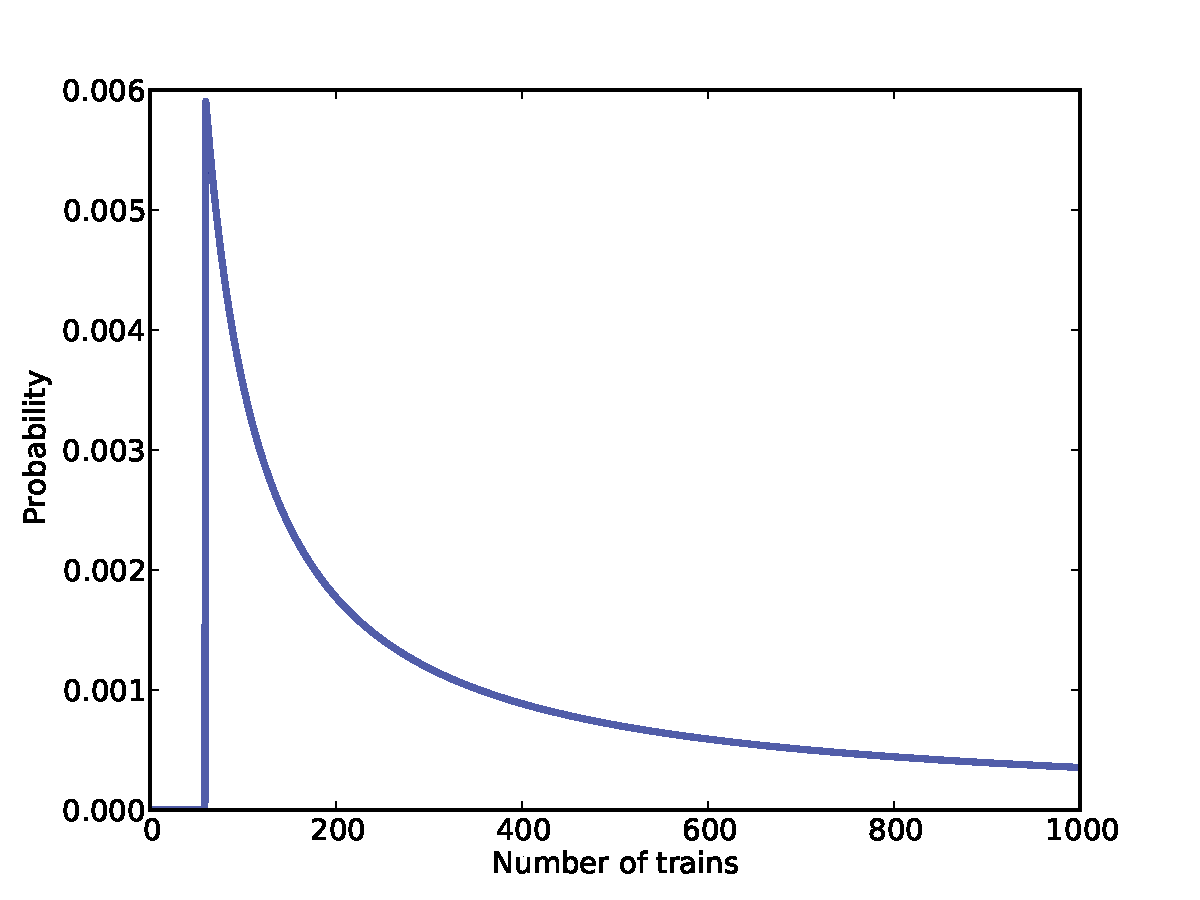
\includegraphics[height=2.5in]{figs/train1.pdf}}
\caption{Posterior distribution for the Locomotive problem, based
on a uniform prior.}
\label{fig.train1}
\end{figure}

The question doesn't give us much basis to choose a prior, but
again we can start with something simple, see what we get, and
then evaluate some alternatives.  So let's assume that $N$ is less
than 1000, and equally likely to be any value from 1 to 1000.

\begin{verbatim}
    hypos = xrange(1, 1001)
    suite = Train(hypos)
\end{verbatim}

Now all we need is a likelihood function.  With a little thought,
you will realize that the likelihood functions for the Locomotive
problem and the Dice problem are identical:

\begin{verbatim}
class Train(Suite):
    def Likelihood(self, hypo, data):
        if hypo < data:
            return 0
        else:
            return 1.0/hypo
\end{verbatim}

And here's the update:

\begin{verbatim}
    suite.Update(60)
\end{verbatim}

Since there are 1000 hypothesis, I didn't print the results.
Instead I used {\tt myplot.Pmf}:

\begin{verbatim}
    myplot.Pmf(suite)
    myplot.Show(xlabel='Number of trains',
                ylabel='Probability')
\end{verbatim}

The result is in Figure~\ref{fig.train1}.  Not surprisingly, all
values of $N$ below 60 have been eliminated.  The most likely
value, if you had to guess, is 60.  That might not seem like
a very good guess; after all, what are the chances that you just
happened to see the train with the highest number?

Nevertheless, if you want to maximize the chance of getting
the answer exactly right, you should guess 60.  But maybe that's
not the right goal.  An obvious alternative is to compute the
mean of the posterior distribution:

\begin{verbatim}
def Mean(suite):
    total = 0
    for hypo, prob in suite.Items():
        total += hypo * prob
    return total

print Mean(suite)
\end{verbatim}

Or you could use the very similar method provided by {\tt Pmf}:

\begin{verbatim}
    print suite.Mean()
\end{verbatim}

The mean of this posterior distribution is 276, so that might be a
good guess if you wanted to minimize error.  If you played this
guessing game over and over, using the mean of the posterior as your
estimate would minimize the total squared error over the long run.

You can download this example from \url{http://thinkbayes.com/train.py}.


\section{What about that prior?}

To make any progress on the Locomotive problem we had to make
some assumptions, and some of them were pretty arbitrary.  In
particular, we chose a uniform prior from 1 to 1000, without
much justification for choosing 1000, or for choosing a uniform
distribution.

It is not crazy to believe that a railroad company might operate
1000 locomotives, but a reasonable person might guess more or fewer.
So we might wonder whether the posterior distribution is sensitive
to these assumptions.  With so little data (only one observation)
it probably is.

Recall that with a uniform prior from 1 to 1000, the mean of
the posterior is 276.  With an upper bound of 500, we get a
posterior mean of 166, and with an upper bound of 2000,
the posterior mean is 467.

So that's bad.  There are two ways to proceed:

\begin{itemize}

\item Get more data.

\item Get more background information.

\end{itemize}

With more data, the posterior distributions based on different
priors tend to converge.  For example, suppose that in addition
to train 60 we also see trains 30 and 90.  We can update the
distribution like this:

\begin{verbatim}
    for data in [60, 30, 90]:
        suite.Update(data)
\end{verbatim}

With these data, the means of the posteriors are

  \begin{tabular}{|l|l|}
  \hline
  Upper & Posterior \\
  Bound & Mean \\
  \hline
  500 & 152 \\
  1000 & 164\\
  2000 & 171\\
  \hline
  \end{tabular}

So the difference between the posteriors is smaller.


\section{An alternative prior}

If more data are not available, another option is to improve the
priors by gathering more background information.  It is probably
not reasonable to assume that a railroad company with 1000 locomotives
is just as likely as a company with only 1.

With some effort, we could probably find a list of companies that
operate locomotives in the area of observation.  Or we could
interview an expert in rail shipping to gather information about
the typical size of companies.

But even without getting into the specifics of railroad economics, we
can make some educated guesses.  In most fields, there are many small
companies, fewer medium-sized companies, and only one or two very
large companies.  In fact, the distribution of company sizes tends to
follow a power law, as Robert Axtell reports in {\it Science} (see
\url{http://www.sciencemag.org/content/293/5536/1818.full.pdf}).

This law suggests that if there are 1000 companies with fewer than
10 locomotives, there might be 100 companies with 100 locomotives,
10 companies with 1000, and possibly one company with 10,000 locomotives.

Mathematically, a power law means the number of companies
with a given size is inversely proportional to the size, or
%
\[ \PMF(x) \propto \left( \frac{1}{x} \right)^{\alpha}   \]
%
where $\PMF(x)$ is the probability mass function of $x$ and $\alpha$ is
a parameter that is often near 1.

We can construct a power law prior like this:

\begin{verbatim}
class Train(Dice):
    def __init__(self, hypos, alpha=1.0):
        Pmf.__init__(self)
        for hypo in hypos:
            self.Set(hypo, hypo**(-alpha))
        self.Normalize()
\end{verbatim}

And here's the code that constructs the prior:

\begin{verbatim}
    hypos = range(1, 1001)
\end{verbatim}

Again, the upper bound is arbitrary, but with a power law
prior, the posterior is less sensitive to this choice.

If we start with this prior and observe trains 30, 60 and 90,
the means of the posteriors are

  \begin{tabular}{|l|l|}
  \hline
  Upper & Posterior \\
  Bound & Mean \\
  \hline
  500 & 131 \\
  1000 & 133 \\
  2000 & 134 \\
  \hline
  \end{tabular}

Now the difference between the posteriors is much smaller.  In fact,
with an arbitrarily large upper bound, the mean converges on 134.

So the power law prior is more realistic, because it is based on
general information about the size of companies, and it
behaves better in practice.

You can download the examples in this section from
\url{http://thinkbayes.com/train3.py}.

\section{Confidence intervals}

Once you have computed a posterior distribution, it is often useful
to summarize the results with a single point estimate or an interval.
For point estimates it is common to use the mean, median, or the
value with maximum likelihood.

For intervals we usually report two values computed
so that there is a 90\% chance that the unknown value falls
between them, or 95\%, or some other value.

These values define a ``confidence interval'' or ``credible interval.''
There is a technical difference between these terms, but I will
use them interchangeably here.

A simple way to compute a confidence interval is to add up the
probabilities in the posterior distribution and record the values
that correspond to probabilities 5\% and 95\%.  In other words,
the 5th and 95th percentiles.

\verb"thinkbayes" provides a function that computes percentiles:

\begin{verbatim}
def Percentile(pmf, percentage):
    p = percentage / 100.0
    total = 0
    for val, prob in pmf.Items():
        total += prob
        if total >= p:
            return val    
\end{verbatim}

And here's the code that uses it:

\begin{verbatim}
    interval = Percentile(suite, 5), Percentile(suite, 95)
    print interval
\end{verbatim}

For the previous example---the locomotive problem with a power law prior
and three trains---the 90\% confidence interval is $(91, 243)$.  The
width of this range suggests, correctly, that we are still quite
uncertain about how many locomotives there are.


\section{Cumulative distribution function}

In the previous section we computed percentiles by iterating through
the values and probabilities in a Pmf.  If we need to compute more
than a few percentiles, it is more efficient to use a cumulative
distribution function, or Cdf.

Cdfs and Pmfs are equivalent in the sense that they contain the
same information about the distribution, and you can always convert
from one to the other.  The advantage of the Cdf is that you can
compute percentiles more efficiently.

{\tt thinkbayes} provides a {\tt Cdf} class that represents a
cumulative distribution function.  It also provides functions for
converting from a Pmf to a Cdf (and back). 

\begin{verbatim}
import thinkbayes
cdf = thinkbayes.MakeCdfFromPmf(suite)
\end{verbatim}

And Cdf provides a function named \verb"Percentile"

\begin{verbatim}
    interval = cdf.Percentile(5), cdf.Percentile(95)
\end{verbatim}

Converting from a Pmf to a Cdf takes time proportional to the number
of values.  The Cdf stores the values and probabilities in sorted
lists, so looking up a probability to get the corresponding value
takes ``log time,'' that is, time proportional to the logarithm of the
number of values.  Looking up a value to get the corresponding
probability is also logarithmic, so Cdfs are efficient for many
calculations.

The examples in this section are in \url{http://thinkbayes.com/train.py}.


\chapter{Urns and Coins}

\section{Four Urns}

James Joyce, the American philosopher not the Irish author, wrote
a paper called {\it How probabilities reflect evidence} that poses
the following problem (which I am quoting loosely):

\begin{quote}
Jacob and Emily both start out knowing that an urn, U, was
randomly chosen from a set of four urns ${urn_0, urn_1, urn_2, urn_3}$
where $urn_i$ contains three balls, $i$ of which are blue and $3-i$ of
which are green. [...]  Jacob and Emily regard random drawing with
replacement as an exchangeable process, so that any series of draws
that produces m blue balls and n green balls is as likely as any other
such series, irrespective of order.  Use $B^m G^n$ to denote the generic
event in which $m$ blue balls and $n$ green balls are drawn at random
and with replacement from U.  Against this backdrop of shared
evidence, suppose Jacob sees five balls drawn at random and with
replacement from U and observes that all are blue, so his evidence is
$B^5 G^0$.  Emily, who sees Jacob's evidence, looks at fifteen additional
draws of which twelve come up blue, so her evidence is $B^{17} G^3$.  [If
$B_{next}$ is the probability that the next ball drawn from the urn is
blue,] what should Emily and Jacob think about $B_{next}$?
\end{quote}

We'll proceed in two steps: the first is to compute the probability
that U is $urn_i$ for each $i$.  The second is to compute $B_{next}$.

Let's use $H_i$ to represent the hypothesis that the urn we chose, U,
is $urn_i$.  Since we are told that U was chosen at random, we can
infer that the prior probabilities are $H_i = 1/4$ for all $i$.

And the likelihood function is easy.  If $H_i$ is true, U contains
$i$ blue balls, so $\p{B|H_i} = i/3$.  Or in Python

\begin{verbatim}
class Urn(Suite):
    def Likelihood(self, hypo, data):
        """
        hypo: integer number of blue balls (out of three)
        data: string 'B' or 'G'
        """
        p = hypo / 3.0
        if data == 'B':
            return p
        else:
            return 1-p
\end{verbatim}

And here's the code that creates the prior and updates it
with Jacob's data:

\begin{verbatim}
    suite = Urn([0,1,2,3])

    for data in 'BBBBB':
        suite.Update(data)
\end{verbatim}

And here are the results:

\begin{verbatim}
0 0.0
1 0.0036231884058
2 0.115942028986
3 0.880434782609
\end{verbatim}

Since he has seen 5 blue and no green balls, Jacob rules out $urn_0$
and gives low posterior probabilities to $urn_1$ and $urn_2$.  Based
on this data, Jacob is 88\% sure that U is $urn_3$.

So what should Jacob believe about $B_{next}$, the chance that the
next ball from U is blue.  If he $H_3$ right, and U is $urn_3$,
then $B_{next}$ is 100\%.  But Jacob is not sure about $H_3$.

Jacob can compute $B_{next}$ using the law of total probability, which
says that the probability that the next ball is blue is the sum
of the probabilities for each way it can happen; in this case
%
\[ B_{next} = \sum \frac{1}{3} \p{H_i | D} \]
%
Pulling out the factor of $1/3$, we have
%
\[ B_{next} = \frac{1}{3} \sum i \p{H_i | D} \]
%
which we recognize as the mean of the posterior distribution, over 3.

\begin{verbatim}
print suite.Mean() / 3.0
\end{verbatim}

For Jacob, $B_{next}$ is 0.96.  For Emily, who sees 17 blue and 3 green
balls, the posterior distribution is 

\begin{verbatim}
0 0.0
1 3.05166468308e-05
2 0.999969483353
3 0.0
\end{verbatim}

Since Emily has seen a blue and a green ball, she can rule out $H_0$
and $H_3$.  And since she has seen many more blue than green balls,
she is all but certain that U is $urn_2$, so her value for $B_{next}$
is very close to 2/3.

Joyce constructed this example to point out a difference between the
evidence seen by Jacob and Emily.  Jacob's evidence has more
``force,'' in one sense of the word, because his posterior belief
about $B_{next}$ is more strongly biased.  But Emily's evidence has
more ``weight,'' because she is more confident about which urn U is.

For Joyce the point of this example is to probe what we mean
when we talk about the ``weight'' or ``force,'' of
evidence.  We come back to this question, from a Bayesian
perspective, in the next chapter.

For us, the point of this example is to provide a warm-up exercise
that will help with the next problem.


\section{The Euro coin problem}
\label{euro}

In {\it Information Theory, Inference, and Learning Algorithms}, David MacKay
poses this question:

\begin{quote}
A statistical statement appeared in ``The Guardian" on Friday January 4, 2002:

  \begin{quote}
        When spun on edge 250 times, a Belgian one-euro coin came
        up heads 140 times and tails 110.  `It looks very suspicious
        to me,' said Barry Blight, a statistics lecturer at the London
        School of Economics.  `If the coin were unbiased, the chance of
        getting a result as extreme as that would be less than 7\%.'
        \end{quote}

But do these data give evidence that the coin is biased rather than fair?
\end{quote}

To answer that question, we'll proceed in two steps.  The first
is to estimate the probability that the coin lands face up.  The second
is to evaluate whether the data support the hypothesis that the
coin is biased.

Any given coin has some probability, $x$, of landing heads up when spun
on edge.  It seems reasonable to believe that the value of $x$ depends
on some physical characteristics of the coin, primarily the distribution
of weight.

If a coin is perfectly balanced, we expect $x$ to be close to 50\%, but
for a lop-sided coin $x$ might be substantially different.  We can use
Bayes's Theorem and the observed data to estimate $x$.

Let's define 101 hypotheses, where $H_i$ is the hypothesis that
$x$ is $i$\%, for values of $i$ from 0 to 100.  I'll start with a uniform
prior where the probability of $H_i$ is the same for all $i$.  We'll
come back later to consider other priors.

\begin{figure}
% euro.py
\centerline{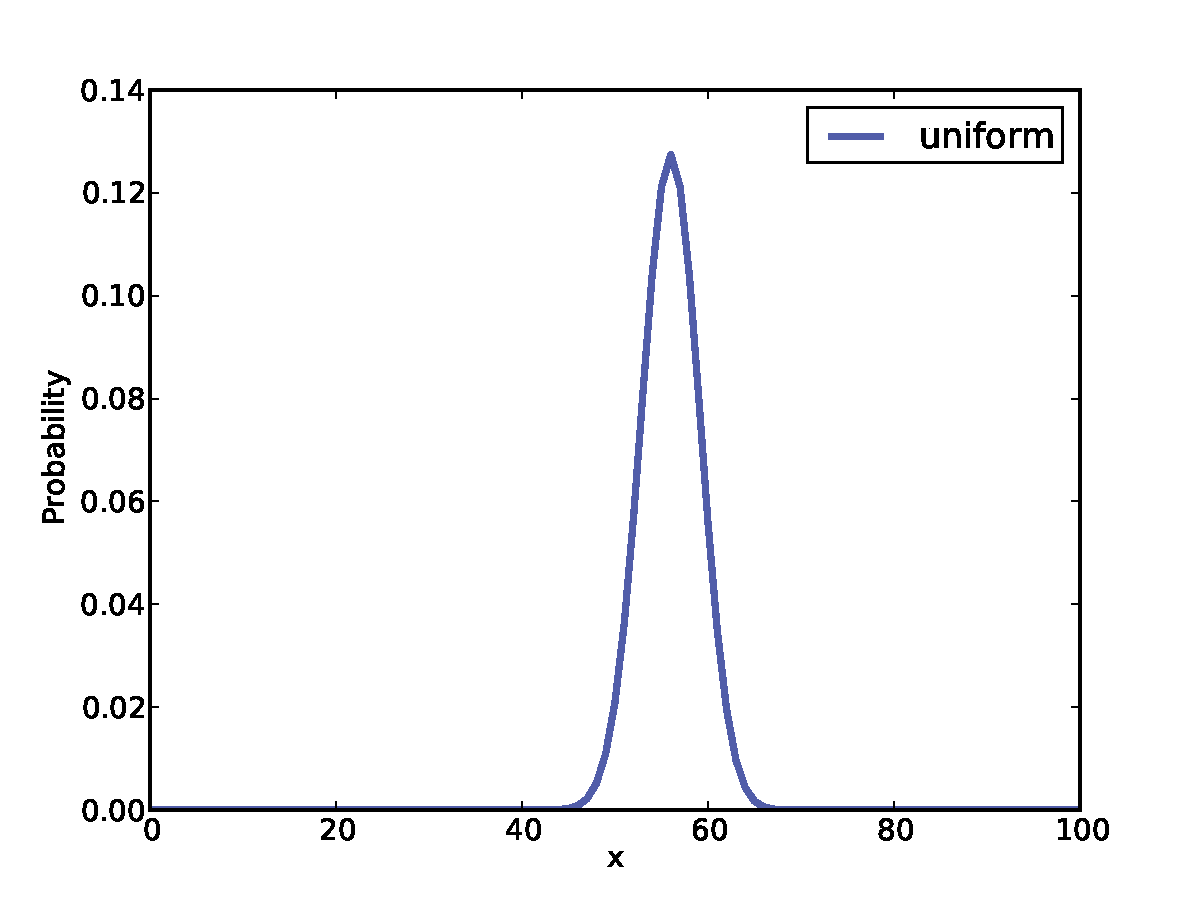
\includegraphics[height=2.5in]{figs/euro1.pdf}}
\caption{Posterior distribution for the Euro problem
on a uniform prior.}
\label{fig.euro1}
\end{figure}

The likelihood function is easy; in fact, it is the same as in
the Four Urn problem.  If $H_i$ is true, then the probability of
heads is $i/100$; the probability of tails is $1- i/100$.

\begin{verbatim}
class Euro(Suite):

    def Likelihood(self, hypo, data):
        x = hypo / 100.0
        if data == 'H':
            return x
        else:
            return 1-x
\end{verbatim}

Here's the code that makes the suite and updates it:

\begin{verbatim}
    suite = Euro(xrange(0, 101))
    dataset = 'H' * 140 + 'T' * 110

    for data in dataset:
        suite.Update(data)
\end{verbatim}

And then we can plot the posterior.

\begin{verbatim}
    myplot.Pmf(suite)
    myplot.Show()
\end{verbatim}

The result is in Figure~\ref{fig.euro1}.


\section{Summarizing the posterior}

Again, there are several ways to summarize the posterior distribution.
One option is to find the most likely value in the posterior
distribution.  \verb"thinkbayes" provides a function that does 
that:

\begin{verbatim}
def MaximumLikelihood(pmf):
    """Returns the value with the highest probability."""
    prob, val = max((prob, val) for val, prob in pmf.Items())
    return val
\end{verbatim}

In this case the result is 56, which is also the observed percentage of
heads, $140/250 = 0.56\%$.  So that suggests (correctly) that the
percentage in a sample is the maximum likelihood estimator
for the population.

We might also summarize the posterior by computing the mean
and median:

\begin{verbatim}
    print 'Mean', suite.Mean()
    print 'Median', thinkbayes.Percentile(suite, 50)
\end{verbatim}

The mean is 55.95; the median is 56.  Finally, we can compute a
confidence interval: 

\begin{verbatim}
    print 'CI', thinkbayes.ConfidenceInterval(suite, 90)
\end{verbatim}

The result is $(51, 61)$.

Now, getting back to the original question,
we would like to know whether the coin is fair.  We observe
that the posterior confidence interval does not include 50\%,
which suggests that the coin is not fair.

But that is not exactly the question we started with.  MacKay asked,
`` Do these data give evidence that the coin is biased rather than
fair?''  To answer that question, we will have to be more precise
about what it means to say that data constitute evidence for
a hypothesis.  And that is the subject of the next chapter.

But before we go, I want to address one possible source of confusion.
Since we want to know whether the coin is fair, it might be tempting
to ask for the probability that {\tt x} is 50\%:

\begin{verbatim}
    print suite.Prob(50)
\end{verbatim}

The result is 0.021, but that value is pretty much meaningless.  The
decision to evaluate 101 hypotheses was arbitrary; we could have
divided the range into more or fewer pieces, and if we had, the
probability for any given hypothesis would be greater or less.


\section{Swamping the priors}

\begin{figure}
% euro.py
\centerline{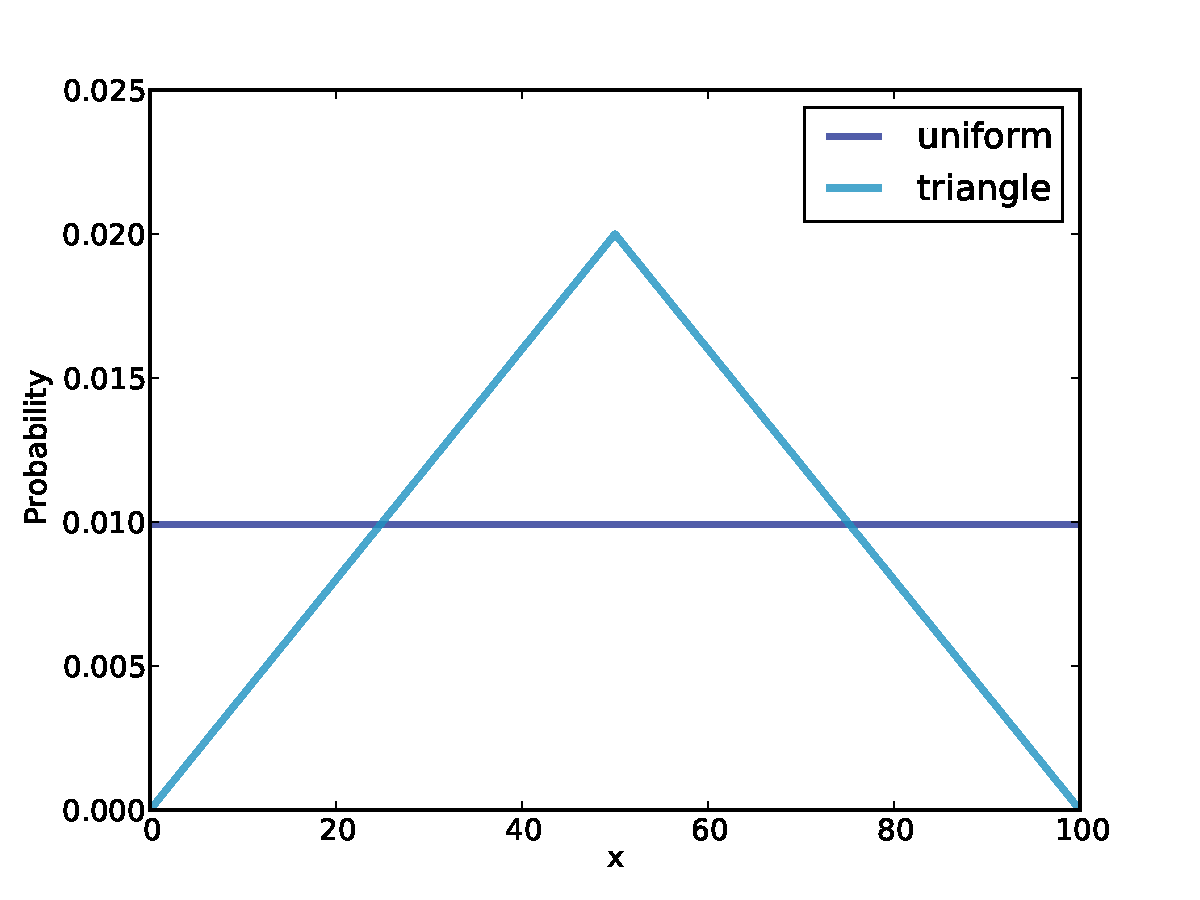
\includegraphics[height=2.5in]{figs/euro2.pdf}}
\caption{Uniform and triangular priors for the
Euro problem.}
\label{fig.euro2}
\end{figure}

\begin{figure}
% euro.py
\centerline{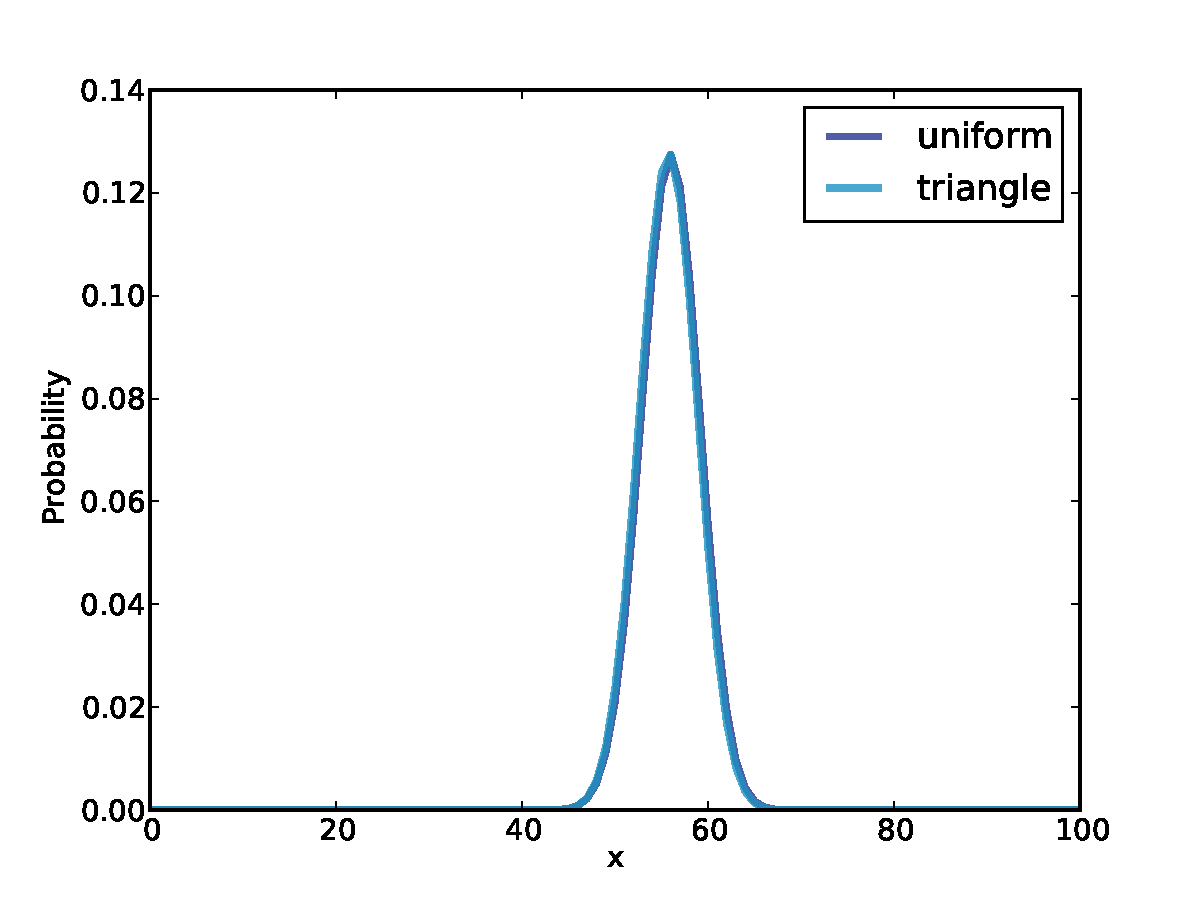
\includegraphics[height=2.5in]{figs/euro3.pdf}}
\caption{Posterior distributions for the Euro problem.}
\label{fig.euro3}
\end{figure}

Again we started with a uniform prior, and again we have to
acknowledge that it was not a very good choice. I can believe
that if a coin is lop-sided, $x$ might deviate substantially from
50\%, but it seems unlikely that the Belgian Euro coin is so
imbalanced that $x$ is 10\% or 90\%.

So it might be more reasonable to choose a prior that gives
higher probability to values of $x$ near 50\% and lower probability
to extreme values.

As an example, I constructed a triangular prior, shown in
Figure~\ref{fig.euro2}.  Here's the code that constructs the prior:

\begin{verbatim}
    suite = Euro(xrange(0, 101))
    for x in range(0, 51):
        suite.Set(x, x)
    for x in range(51, 101):
        suite.Set(x, 100-x) 
    suite.Normalize()
\end{verbatim}

Figure~\ref{fig.euro2} shows the result.  Updating this prior
with the same dataset yields the posterior distribution shown
in Figure~\ref{fig.euro3}.

The point of this example is that even with substantially different
priors, the posterior distributions are very similar.  The medians
and the confidence intervals are identical; the means differ by
less than 0.5\%.

This is an example of ``swamping the priors:'' with enough
data, people who start with different priors will tend to
converge on the same posterior.


\section{Optimization}

The code I have shown so far is meant to be easy to read, but it
is not very efficient.  In general, I like to develop code that
is demonstrably correct, then check whether it is fast enough for
my purposes.  If so, there is no need to optimize.
For this example, if we care about run time,
there are several ways we can speed it up.

The first opportunity is to reduce the number of times we
normalize the suite.
In the original code, we call \verb"Update" once for each spin.

\begin{verbatim}
    dataset = 'H' * heads + 'T' * tails

    for data in dataset:
        suite.Update(data)
\end{verbatim}

And here's what \verb"Update" looks like:

\begin{verbatim}
    def Update(self, data):
        for hypo in self.Values():
            like = self.Likelihood(hypo, data)
            self.Mult(hypo, like)
        return self.Normalize()
\end{verbatim}

Each update iterates through the hypotheses, then calls \verb"Normalize",
which iterates through the hypotheses again.  We can save some
time by doing all of the updates before normalizing.

\verb"Suite" provides a method called \verb"UpdateSet" that does
exactly that.  Here it is:

\begin{verbatim}
    def UpdateSet(self, dataset):
        for data in dataset:
            for hypo in self.Values():
                like = self.Likelihood(hypo, data)
                self.Mult(hypo, like)
        return self.Normalize()
\end{verbatim}

And here's how we can invoke it:

\begin{verbatim}
    dataset = 'H' * heads + 'T' * tails
    suite.UpdateSet(dataset)
\end{verbatim}

This optimization speeds things up, but the run time is still
proportional to the amount of data.  We can speed things up
even more by rewriting \verb"Likelihood" to process the entire
dataset, rather than one spin at a time.

In the original version,
\verb"data" is a string that encodes either heads or tails:

\begin{verbatim}
    def Likelihood(self, hypo, data):
        x = hypo / 100.0
        if data == 'H':
            return x
        else:
            return 1-x
\end{verbatim}

As an alternative, we could encode the dataset as a tuple of 
two integers: the number of heads and tails.
In that case \verb"Likelihood" looks like this:

\begin{verbatim}
    def Likelihood(self, hypo, data):
        x = hypo / 100.0
        heads, tails = data
        like = x**heads * (1-x)**tails
        return like
\end{verbatim}

And then we can call \verb"Update" like this:

\begin{verbatim}
    heads, tails = 140, 110
    suite.Update((heads, tails))
\end{verbatim}

Since we have replaced repeated multiplication with exponentiation,
this version takes the same time for any number of spins (up
to a point).

For this example there is yet another optimization we can apply,
but we'll come back to that later.


\chapter{Odds and addends}

\section{Odds}

One way to represent a probability is with a number between
0 and 1, but that's not the only way.  If you have ever bet
on a football game or a horse race, you have probably encountered
another representation of probability, called ``odds.''

You might have heard expressions like ``the odds are
three to one against,'' but you might not know what they mean.  
The odds in favor of an event are the ratio of the probability
it will occur to the probability that it will not.

So if I think my team has a 75\% chance of winning, I would
say that the odds in their favor are three to one, because
the chance of winning is three times the chance of losing.

You can write odds in decimal form, but it is most common to
write them as a ratio of integers.  So ``three to one'' is
written $3:1$.

When probabilities are low, it is more common to report the
``odds against'' rather than the odds in favor.  For
example, if I think my horse has a 10\% chance of winning,
I would say that the odds against are $9:1$.

In the context of betting, it can be confusing to talk about
odds, because the same format is used to report the payoff.
For example, if I offer you a bet with a payoff of ``two to one,''
that means I will pay you \$2 for every \$1 you bet (if
you win).  Of course, I would only offer you that bet if
I thought the odds against you were more than $2:1$.

But this is not a book about gambling, so I will only talk about odds
and forget about payoffs.

Probabilities and odds are different representations of the
same information.  Given a probability, you can compute the
odds like this:

\begin{verbatim}
def Odds(p):
    return p / (1-p)
\end{verbatim}

Given the odds in favor, in decimal form, you can convert to
probability like this:

\begin{verbatim}
def Probability(o):
    return o / (o+1)
\end{verbatim}

If you represent odds with a numerator and denominator, you
can convert to probability like this:

\begin{verbatim}
def Probability2(yes, no):
    return yes / (yes + no)
\end{verbatim}

When I work with odds in my head, I find it helpful to picture
people at the track.  If 20\% of them think my horse will win,
then 80\% of them don't, so the odds in favor are $20:80$ or
$1:4$.

If the odds are $5:1$ against my horse, then five out of six
people think she will lose, so the probability of winning
is $1/6$.

\section{The odds form of Bayes's Theorem}

In Chapter~\ref{intro} I wrote Bayes's Theorem in the ``probability
form'':
%
\[ \p{H|D} = \frac{\p{H}~\p{D|H}}{\p{D}} \]
%
If we define $\bar{H}$ as ``hypothesis H is false'', we can write the
odds in favor of $H$ like this:
%
\[ \frac{\p{H|D}}{\p{\bar{H}|D}} = \frac{\p{H}~\p{D|H}}
                                        {\p{\bar{H}}~\p{D|\bar{H}}} \]
%
Or writing \o{H} for odds in favor of H:
%
\[ \o{H|D} = \o{H} \frac{\p{D|H}}{\p{D|\bar{H}}} \]
%
In words, this says that the posterior odds are the prior odds times
the likelihood ratio.  This is the ``odds form'' of Bayes's Theorem.

This form is most convenient for computing a Bayesian update on
paper, or in your head.  For example, let's go back to the
cookie problem:

\begin{quote}
Suppose there are two bowls of cookies.  Bowl 1 contains
  30 vanilla cookies and 10 chocolate cookies.  Bowl 2 contains 20 of
  each.

Now suppose you choose one of the bowls at random and, without looking,
select a cookie at random.  The cookie is vanilla.  What is the probability
that it came from Bowl 1?
\end{quote}

The prior probability is 50\%, so the prior odds are $1:1$, or just
$1$.  The likelihood ratio is $\frac{3}{4} / \frac{1}{2}$, or $3/2$.
So the posterior odds are $3:2$, which corresponds to probability
$3/5$.


\section{Oliver's blood}
\label{evidence}

Here is another problem from MacKay's {\it Information Theory,
  Inference, and Learning Algorithms}:

\begin{quote}
Two people have left traces of their own blood at the scene of
a crime.  A suspect, Oliver, is tested and found to have type
'O' blood.  The blood groups of the two traces are found to
be of type 'O' (a common type in the local population, having frequency
60\%) and of type 'AB' (a rare type, with frequency 1\%).
Do these data [the traces found at the scene] give evidence
in favor of the proposition that Oliver was one of the people
[who left blood at the scene]?
\end{quote}

To answer this question, we need to think about what it means
for data to give evidence in favor of (or against) a hypothesis.
Intuitively, we might say that data favor a hypothesis if the
hypothesis is more likely in light of the data than it was before.

In the cookie problem, the prior odds are $1:1$, or probability 50\%.
The posterior odds are $3:2$, or probability 60\%.  So we could say
that the vanilla cookie is evidence in favor of Bowl 1.

The odds form of Bayes's Theorem provides a way to make this
intuition more precise.  Again
%
\[ \o{H|D} = \o{H} \frac{\p{D|H}}{\p{D|\bar{H}}} \]
%
Or dividing through by \o{H}:
%
\[ \frac{\o{H|D}}{\o{H}} = \frac{\p{D|H}}{\p{D|\bar{H}}} \]
%
The term on the left is the ratio of the posterior and prior odds.
The term on the right is the likelihood ratio, also called the ``Bayes
factor.

If the Bayes factor value is greater than $1$, that means that the
data were more likely under $H$ than under $\bar{H}$.  And since the
odds ratio is also greater than $1$, that means that the odds are
greater, in light of the data, than they were before.

If the Bayes factor is less than $1$, that means the data were
less likely under $H$ than under $\bar{H}$, so the odds in
favor of $H$ go down.

Finally, if the Bayes factor is exactly $1$, the data are equally
likely under either hypothesis, so the odds do not change.

Now we can get back to the Oliver's blood problem.  If Oliver is
one of the people who left blood at the crime scene, then he
accounts for the 'O' sample, so the probability of the data
is just the probability that a random member of the population
has type 'AB' blood, which is 1\%.

If Oliver did not leave blood at the scence, then we have two
samples to account for.  If we choose two random people from
the population, what is the chance of finding one with type 'O'
and one with type 'AB'?  Well, there are two ways it might happen:
the first person we choose might have type 'O' and the second
'AB', or the other way around.  So the total probability is
$2 (0.6) (0.01)\ = 1.2\%$.

The likelihood of the data is slightly higher if Oliver is
{\it not} one of the people who left blood at the scence, so
the blood data is actually evidence against Oliver's guilt.

This example is a little contrived, but it is an example of
the counterintuitive result that data {\it consistent} with
a hypothesis are not necessarily {\it in favor of}
the hypothesis.

If this result is so counterintuitive that it bothers you,
this way of thinking might help: the data consist of a common
event, type 'O' blood, and a rare event, type 'AB' blood.
If Oliver accounts for the common event, that leaves the rare
event still unexplained.  If Oliver doesn't account for the
'O' blood, then we have two chances to find someone in the
population with 'AB' blood.  And that factor of two makes
the difference.

\section{Addends}

Dungeons and Dragons is a role-playing game where the results
of players' decisions are usually determined by rolling dice.
In fact, before game play starts, players generate each
attribute of their characters---strength, intelligence, wisdom,
dexterity, constitution, and charisma---by rolling three
six-sided dice and adding them up.

So you might be curious to know the distribution of this sum.
There are two ways you might compute it:

\begin{description}

\item[Simulation:] Given a Pmf that represents the distribution
for a single die, you can draw random samples, add them up,
and accumulate the distribution of simulated sums.

\item[Convolution:] Given two Pmfs, you can enumerate all possible
pairs of values and compute the distribution of the sums.

\end{description}

\verb"thinkbayes" provides functions for both.  Here's an example
of the first approach.  First, I'll define a class to represent
a single die as a Pmf:

\begin{verbatim}
class Die(thinkbayes.Pmf):
    def __init__(self, sides):
        d = dict((i, 1) for i in xrange(1, sides+1))
        thinkbayes.Pmf.__init__(self, d)
        self.Normalize()
\end{verbatim}

Now I can create a six-sided die:

\begin{verbatim}
    d6 = Die(6)
\end{verbatim}

And use \verb"SampleSum" to generate a sample of 1000 rolls.

\begin{verbatim}
    dice = [d6] * 3
    three = thinkbayes.SampleSum(dice, 1000)
\end{verbatim}

\verb"SampleSum" is based on another function, \verb"RandomSum",
also in \verb"thinkbayes.py":

\begin{verbatim}
def RandomSum(dists):
    total = sum(dist.Random() for dist in dists)
    return total


def SampleSum(dists, n):
    pmf = MakePmfFromList(RandomSum(dists) for i in xrange(n))
    return pmf
\end{verbatim}

\verb"dists" is a list of objects that can be either
Pmfs or Cdfs (or anything else that provides an appropriate
\verb"Random" method); \verb"n" is the number of rolls to simulate.

The drawback of estimating this distribution by simulation is that
it is only approximately correct.  As \verb"n" gets larger, it gets
more accurate, but of course the run time increases as well.

The other approach is to enumerate all pairs of values and
compute the sum and probability of each pair.  This is implemented
in the \verb"Pmf.__add__" method:

\begin{verbatim}
    def __add__(self, other):
        pmf = Pmf()
        for v1, p1 in self.Items():
            for v2, p2 in other.Items():
                pmf.Incr(v1+v2, p1*p2)
        return pmf
\end{verbatim}

And here's how it's used:

\begin{verbatim}
    three_exact = d6 + d6 + d6
\end{verbatim}

The approximate and exact distributions are shown in
Figure~\ref{fig.dungeons1}.

\begin{figure}
% dungeons.py
\centerline{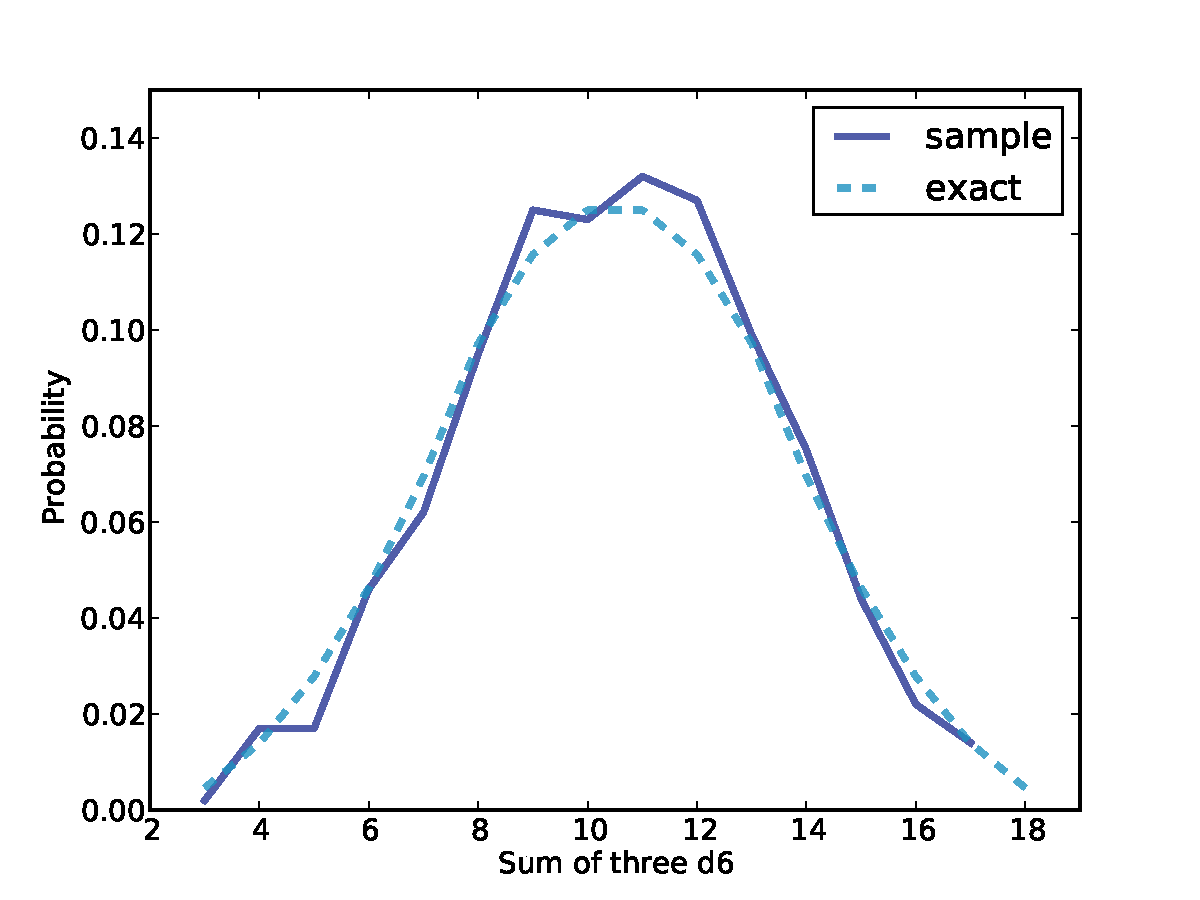
\includegraphics[height=2.5in]{figs/dungeons1.pdf}}
\caption{Approximate and exact distibutions for the sum of
three six-sided dice.}
\label{fig.dungeons1}
\end{figure}

\verb"Pmf.__add__" is based on the assumption that the random
selections from each Pmf are independent.  In the example of rolling
several dice, this assumption is pretty good.  In other cases, we
might have to extend this method to use conditional probabilities.

The code from this section is available from
\url{http://thinkbayes.com/dungeons.py}.


\section{Maxima}

Having generated a Dungeons and Dragons character, I would be
particularly interested in the character's best attributes, so
I might wonder what is the chance of getting an 18 in one or
more attributes, or more generally what is the
distribution of the best attribute.

There are three ways to compute the distribution of a maximum:

\begin{description}

\item[Simulation:] Given a Pmf that represents the distribution
for a single selection, you can a random samples, find the maximum,
and accumulate the distribution of simulated maxima.

\item[Convolution:] Given two Pmfs, you can enumerate all possible
pairs of values and compute the distribution of the maxima.

\item[Exponentiation:] If we convert a Pmf to a Cdf, there is a simple
and efficient algorithm for finding the Cdf of the maxima.

\end{description}

The code to simulate maxima is almost identical to the code for
simulating sums:

\begin{verbatim}
def RandomMax(dists):
    total = max(dist.Random() for dist in dists)
    return total


def SampleMax(dists, n):
    pmf = MakePmfFromList(RandomMax(dists) for i in xrange(n))
    return pmf
\end{verbatim}

All I did was replace ``sum'' with ``max''.  And the code
for convolution is almost identical, too:

\begin{verbatim}
def PmfMax(pmf1, pmf2):
    res = thinkbayes.Pmf()
    for v1, p1 in pmf1.Items():
        for v2, p2 in pmf2.Items():
            res.Incr(max(v1, v2), p1*p2)
    return res
\end{verbatim}

In fact, you could generalize this function by taking the
appropriate operator as a parameter.

The only problem with this algorithm is that if each Pmf
has $n$ values, the run time is proportional to $n^2$.

If we convert the Pmfs to Cdfs, we can do the same calculation
in linear time!  The key is to remember the definition of the
cumulative distribution function:
%
\[ CDF(x) = \p{X \le x} \]
%
where $X$ is a random variable that means ``a value chosen
randomly from this distribution.''  So, for example, $CDF(5)$
is the probability that a value from this distribution is less
than or equal to 5.

If I draw $X$ from $CDF_1$ and $Y$ from $CDF_2$, and compute
the maximum $Z = max(X, Y)$, what is the chance that $Z$ is
less than or equal to 5?  Well, in that case both $X$ and $Y$
must be less than or equal to 5.

If the selections of $X$ and $Y$ are independent,
%
\[ CDF_3(5) = CDF_1(5) CDF_2(5) \] 
%
where $CDF_3$ is the distribution of $Z$.  I chose the value
5 because I think it makes the formulas easy to read, but we
can generalize for any value of $z$:
%
\[ CDF_3(z) = CDF_1(z) CDF_2(z) \]
%
In the special case where we draw $n$ values from the same
distribution, 
%
\[ CDF_n(z) = CDF_1(z)^n \]
%
And \verb"Cdf" provides a method that does just that:

\begin{verbatim}
    def Max(self, n):
        cdf = self.Copy()
        cdf.ps = [p**n for p in cdf.ps]
        return cdf
\end{verbatim}

\verb"Max" takes the sample size, {\tt n}, and returns a new
Cdf that represents the distribution of the maximum of {\tt n}
values.

\verb"Pmf.Max" does the same thing for Pmfs.  It has to
do a little more work to convert the Pmf to a Cdf, so the
run time is proportional to $n \log n$, but that's still
better than quadratic.

Finally, here's an example that computes the distribution of
your character's best attribute:

\begin{verbatim}
    best_attr_cdf = three_exact.Max(6)
    best_attr_pmf = thinkbayes.MakePmfFromCdf(best_attr_cdf)
\end{verbatim}

Where \verb"three_exact" is defined in the previous section.
If we print the results, we see that the chance of generating
a character with at least one attribute of 18 is about 3\%.

[[[Include the figure.]]]


\chapter{Hockey}

\section{The Boston Bruins problem}

In the 2010-11 National Hockey League (NHL) Finals, my beloved Boston
Bruins played a best-of-seven championship series against the despised
Vancouver Canucks.  Boston lost the first two games 0-1 and 2-3, then
won the next two games 8-1 and 4-0.  At this point in the series, what
is the probability that Boston will win the next game, and what is
their probability of winning the championship?

As always, to answer a question like this, we need to make some
assumptions.  First, it is reasonable to believe that goal scoring in
hockey is at least approximately a Poisson process, which means that
it is equally likely for a goal to be scored at any time during a
game.  Second, we can assume that when team A plays team B, each team
has some long-term average goals per game, denoted $\lambda$.

Given these assumptions, my strategy for answering this question is

\begin{enumerate}

\item Use statistics from previous games to choose a prior
distribution for $\lambda$.

\item Use the score from the first four games to estimate $\lambda$
for each team.

\item Use the posterior distributions of $\lambda$ to compute 
distribution of goals for each team, the distribution of the
goal differential, and the probability that each team wins.

\item Simulate the rest of the series to estimate the probability
of each possible outcome.

\end{enumerate}

To choose a prior distribution, I got some statistics from
\url{http://www.nhl.com}, specifically the average goals per game
for each team in the 2010-11 season.  The distribution is roughly
normal (Gaussian) with mean 2.8 and standard deviation 0.3.

The Gaussian distribution is continuous, but we'll approximate it with
a discrete Pmf.  \verb"thinkbayes" provides \verb"MakeGaussianPmf" to
do exactly that:

\begin{verbatim}
def MakeGaussianPmf(mu, sigma, num_sigmas, n=101):
    pmf = Pmf()
    low = mu - num_sigmas*sigma
    high = mu + num_sigmas*sigma

    for x in numpy.linspace(low, high, n):
        p = EvalGaussianPdf(mu, sigma, x)
        pmf.Set(x, p)
    pmf.Normalize()
    return pmf
\end{verbatim}  

{\tt mu} and {\tt sigma} are the mean and standard deviation of the
Gaussian distribution.  \verb"num_sigmas" is the number of standard
deviations above and below the mean that the Pmf will span, and {\tt
  n} is the number of values in the Pmf.

\verb"EvalGaussianPdf" does what it says; it evaluates the
Gaussian probability density function (PDF).

\begin{verbatim}
def EvalGaussianPdf(mu, sigma, x):
    z = (x - mu) / sigma
    p = math.exp(-z**2/2)
    return p
\end{verbatim}  

If you look up the Gaussian PDF, you'll see that I left out a
normalizing constant, so this function actually computes
a likelihood that is proportional to the Gaussian PDF.  But
that's fine, because I have to normalize the Pmf anyway.

Getting back to the hockey problem, here's the definition for a suite
of hypotheses about the value of $\lambda$.

\begin{verbatim}
class Hockey(thinkbayes.Suite):

    def __init__(self):
        thinkbayes.Suite.__init__(self)

        pmf = thinkbayes.MakeGaussianPmf(2.7, 0.3, 6)
        for x, p in pmf.Items():
            self.Set(x, p)
\end{verbatim}  

So the prior distribution is Gaussian with mean 2.7, standard deviation
0.3, and it spans six sigmas above and below the mean.

As always, we have to decide how to represent each hypothesis; in
this case I represent the hypothesis that $\lambda=x$ with the
floating-point value {\tt x}. 


\section{Poisson processes}

In mathematical statistics, a ``process'' is a stochastic, or random,
model of a physical system.  For example, a Bernoulli process is a model
of a sequence of events, called trials, in which each trial has
two possible outcomes, like success and failure.  So a Bernoulli
process is a natural model for a series of coin flips, or a series
of shots on goal.

A Poisson process is the continuous version of a Bernoulli process,
where an event can occur at any point in time with equal probability.
Poisson processes can be used to model customers arriving in a store,
buses arriving at a bus stop, or goals scored in a hockey game.

In many real systems the probability of an event changes over time.
Customers are more likely to go to a store at certain times of day,
buses are supposed to arrive at fixed intervals, and goals are more
or less likely at different times during a game.

But all models are based on simplifications, and in this case modeling
a hockey game with a Poisson process is a reasonable choice.  Heuer
et al. analyze scoring in a German soccer league and come to the same
conclusion; see
\url{http://www.cimat.mx/Eventos/vpec10/img/poisson.pdf}.

The benefit of using this model is that we can compute the distribution
of goals per game efficiently, as well as the distribution of time
between goals.  Specifically, if the average number of goals
in a game is {\tt lam}, the distribution of goals per game is
given by the Poisson PMF:

\begin{verbatim}
def EvalPoissonPmf(lam, k):
    return (lam)**k * math.exp(-lam) / math.factorial(k)
\end{verbatim}  

And the distribution of time between goals is given by the
exponential PDF:

\begin{verbatim}
def EvalExponentialPdf(lam, x):
    return lam * math.exp(-lam * x)
\end{verbatim}  

I use the variable
{\tt lam} because {\tt lambda} is a reserved keyword in Python.
Both of these functions are in \verb"thinkbayes.py".


\section{The posteriors}

Now we can compute the likelihood of seeing a team with a hypothetical
value of {\tt lam} score {\tt k} goals in a game:

\begin{verbatim}
# class Hockey

    def Likelihood(self, hypo, data):
        lam = hypo
        k = data
        like = thinkbayes.EvalPoissonPmf(lam, k)
        return like
\end{verbatim}

Each hypothesis is a possible value of $\lambda$;  {\tt
  data} is the observed number of goals, {\tt k}.

With the likelihood function in place, we can make a suite for each
team and update them with the scores from the first four games.

\begin{verbatim}
    suite1 = Hockey('bruins')
    suite1.UpdateSet([0, 2, 8, 4])
     
    suite2 = Hockey('canucks')
    suite2.UpdateSet([1, 3, 1, 0])
\end{verbatim}  

Figure~\ref{fig.hockey1} shows the resulting posterior distributions
for {\tt lam}.  Based on the first four games, the most likely
values for {\tt lam} are 2.6 for the Canucks and 2.9 for the Bruins.

\begin{figure}
% hockey.py
\centerline{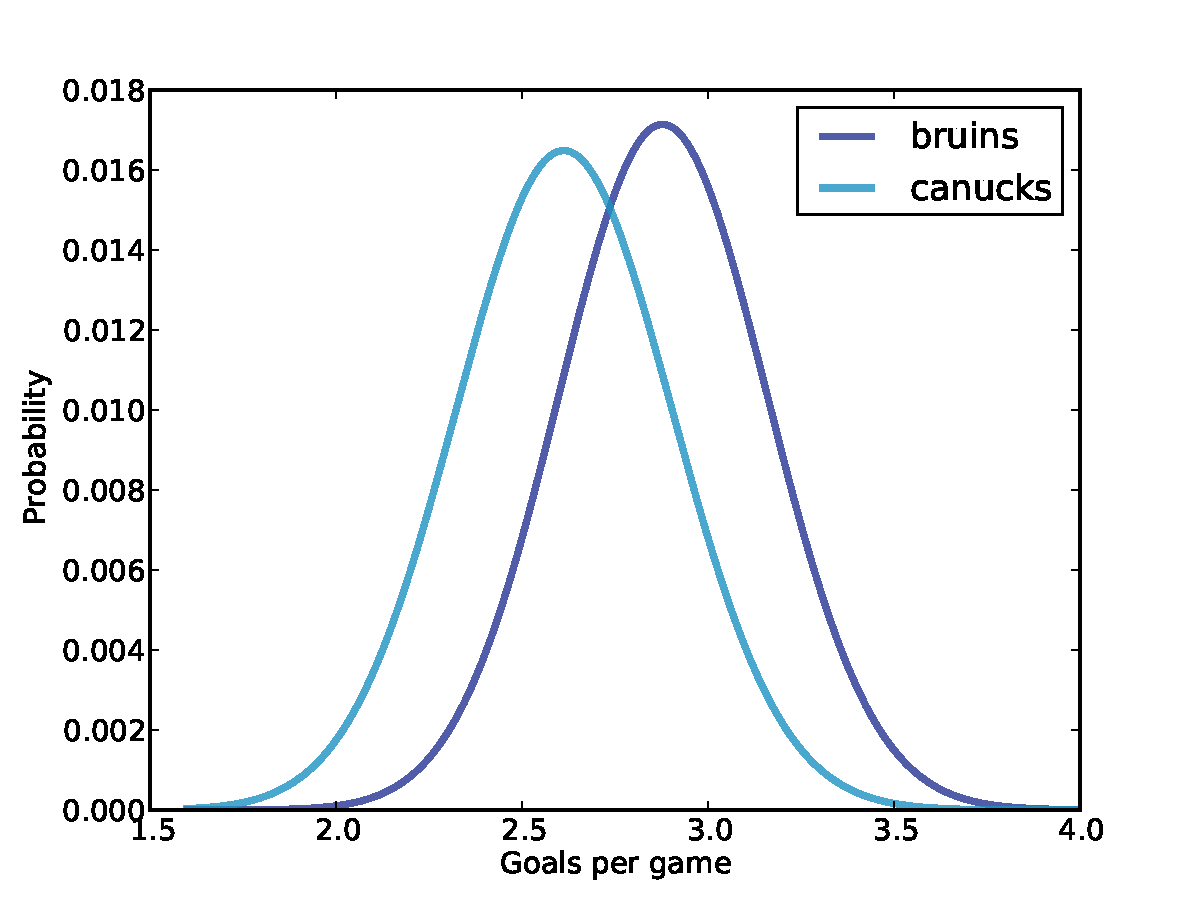
\includegraphics[height=2.5in]{figs/hockey1.pdf}}
\caption{Posterior distribution of the number of
goals per game.}
\label{fig.hockey1}
\end{figure}

\begin{figure}
% hockey.py
\centerline{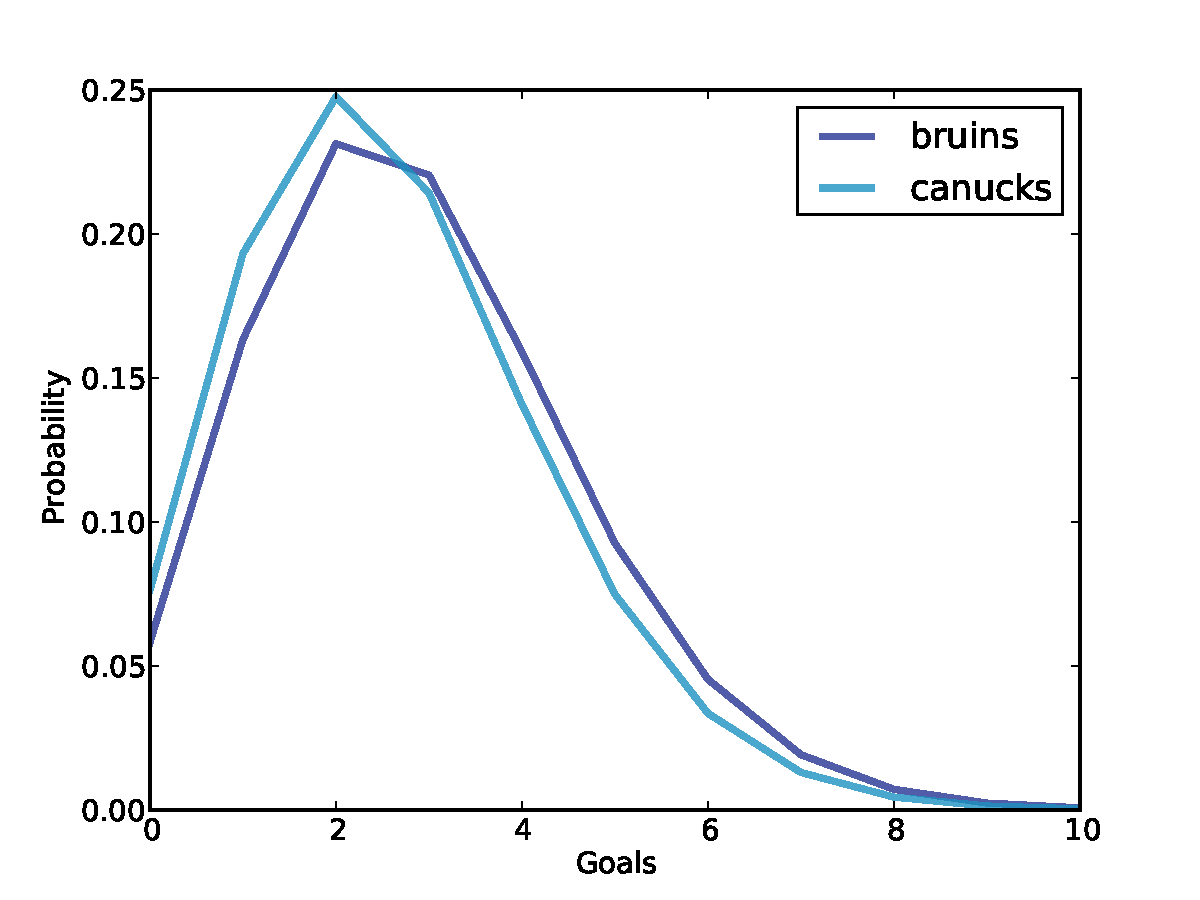
\includegraphics[height=2.5in]{figs/hockey2.pdf}}
\caption{Distribution of goals in a single game.}
\label{fig.hockey2}
\end{figure}

\begin{figure}
% hockey.py
\centerline{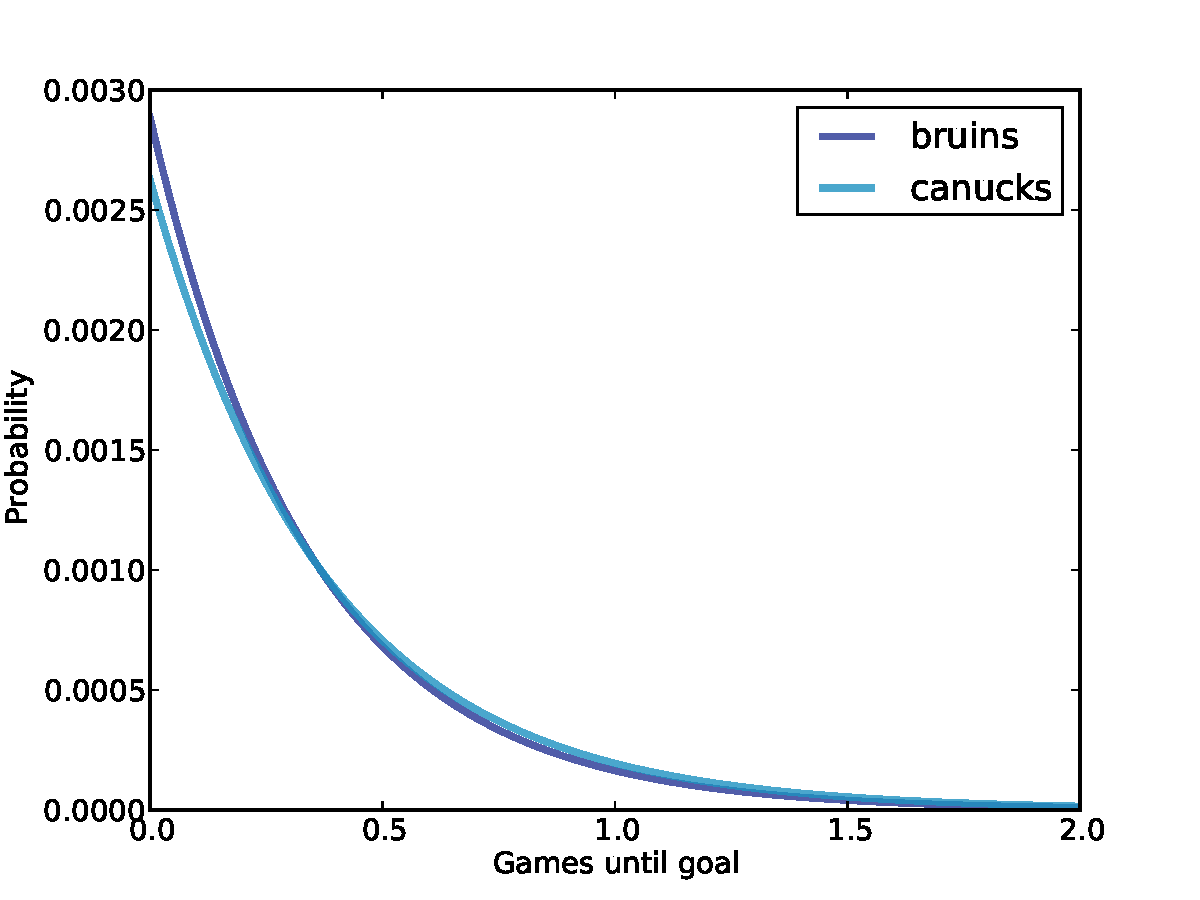
\includegraphics[height=2.5in]{figs/hockey3.pdf}}
\caption{Distribution of time between goals.}
\label{fig.hockey3}
\end{figure}


\section{The Meta-Pmf}

To compute the probability that each team wins the next game,
we need to compute the distribution of goals for each team.

If we knew the value of {\tt lam} exactly, we could use the
Poisson distribution again.  \verb"thinkbayes" provides a
method that computes a truncated approximation of a Poisson
distribution:

\begin{verbatim}
def MakePoissonPmf(lam, high):
    pmf = Pmf()
    for k in xrange(0, high+1):
        p = EvalPoissonPmf(lam, k)
        pmf.Set(k, p)
    pmf.Normalize()
    return pmf
\end{verbatim}  

The range of values in the computed Pmf is from 0 to {\tt high}.
So if the value of {\tt lam} were exactly 3.4, we would compute:

\begin{verbatim}
lam = 3.4
goal_dist = thinkbayes.MakePoissonPmf(lam, 10)
\end{verbatim}

I chose the upper bound, 10, because the probability of scoring
more than 10 goals in a game is quite low.

That's simple enough so far; the problem is that we don't know
the value of {\tt lam} exactly.  Instead, we have a distribution
of possible values for {\tt lam}.

For each value of {\tt lam}, the distribution of goals is Poisson.
So the overall distribution of goals is a mixture of these
Poisson distributions, weighted according to the probabilities
in the distribution of {\tt lam}.

\verb"thinkbayes" provides a method that computes mixtures
of distributions:

\begin{verbatim}
def MakeMixture(metapmf):
    mix = Pmf()
    for pmf, p1 in metapmf.Items():
        for x, p2 in pmf.Items():
            mix.Incr(x, p1 * p2)
    return mix
\end{verbatim}  

{\tt metapmf} is a Meta-Pmf, which means that it is a Pmf that
contains Pmfs.  If you find the Meta-Pmf confusing; it might
help to think about how you would generate a random value from
a Meta-Pmf.  First you would choose a Pmf according to the
probabilities in the Meta-Pmf.  Then you would choose a value
according to the probabilities in the chosen Pmf.

\verb"MakeMixture" computes the distribution of the resulting
values.

Given the posterior distribution of {\tt lam}, here's the code
that makes the distribution of goals:

\begin{verbatim}
def MakeGoalPmf(suite):
    metapmf = thinkbayes.Pmf()
    high = 10

    for lam, prob in suite.Items():
        pmf = thinkbayes.MakePoissonPmf(lam, high)
        metapmf.Set(pmf, prob)

    mix = thinkbayes.MakeMixture(metapmf)
    return mix
\end{verbatim}  

For each value of {\tt lam} we make a Poisson Pmf and add it to the
Meta-Pmf.  Then we use \verb"MakeMixture" to compute the mixture.  If
the Meta-Pmf makes your head hurt, don't panic.  We are past the hard
part of the problem now; everything else is easy.

Figure~\ref{fig.hockey2} shows the resulting distribution of goals for
the Bruins and Canucks.  As expected, the Bruins are less likely to
score 3 goals or fewer in the next game, and more likely to score 4 or
more.

\section{The probability of winning}

To get the probability of winning, we can convolve the distributions
from the previous section to get the distribution of the goal
differential:

\begin{verbatim}
    goal_dist1 = MakeGoalPmf(suite1)
    goal_dist2 = MakeGoalPmf(suite2)
    diff = goal_dist1 - goal_dist2
\end{verbatim}  

If this differential is positive, the Bruins win; if negative,
the Canucks win; if 0, it's a tie:

\begin{verbatim}
    p_win = diff.ProbGreater(0)
    p_loss = diff.ProbLess(0)
    p_tie = diff.Prob(0)
\end{verbatim}  

With the distributions from the previous section, \verb"p_win"
is 46\%, \verb"p_loss" is 37\%, and \verb"p_tie" is 17\%.

In the event of a tie at the end of regulation play, the teams play
overtime periods until one team scores.  Since the game ends
immediately when the first goal is scored, this overtime format
is known as ``sudden death.''


\section{Sudden death}

To compute the probability of winning in a sudden death overtime,
the important statistic is not goals per game, but time until the
first goal.  The assumption that goal-scoring is a Poisson process
is helpful here, because it implies that the time between goals
is exponentially distributed.

Given {\tt lam}, we can compute the time between goals like this: 

\begin{verbatim}
lam = 3.4
time_dist = thinkbayes.MakeExponentialPmf(lam, high=2, n=101)
\end{verbatim}  

{\tt high} is the upper bound of the distribution.  In this case
I chose 2, because the probability of going more than two games
without scoring is small.  {\tt n} is the number of values in
the Pmf.

If we know {\tt lam} exactly, that's all there is to it.
But we don't; instead we have a posterior
distribution of possible values.  So as we did with the distribution
of goals, we have to make a Meta-Pmf and compute a mixture of
Pmfs.

\begin{verbatim}
def MakeGoalTimePmf(suite):
    metapmf = thinkbayes.Pmf()

    for lam, prob in suite.Items():
        pmf = thinkbayes.MakeExponentialPmf(lam, high=2, n=2001)
        metapmf.Set(pmf, prob)

    mix = thinkbayes.MakeMixture(metapmf)
    return mix
\end{verbatim}  

Figure~\ref{fig.hockey2} shows the resulting distributions.  For
time values less than one period (one third of a game), the Bruins
are more likely to score.  The time until the Canucks score is
more likely to be longer.

I set the number of values, {\tt n},
fairly high in order to minimize the number of ties, since it is not
actually possible for both teams to score simultaneously.

Now we can compute the probability that the Bruins score first:

\begin{verbatim}
    time_dist1 = MakeGoalTimePmf(suite1)
    time_dist2 = MakeGoalTimePmf(suite2)
    p_overtime = thinkbayes.PmfProbLess(time_dist1, time_dist2)
\end{verbatim}  

For the Bruins, the probability of winning in overtime is 52\%.
Finally, we can compute the total probability of winning:

\begin{verbatim}
    p_tie = diff.Prob(0)
    p_overtime = thinkbayes.PmfProbLess(time_dist1, time_dist2)

    p_win = diff.ProbGreater(0) + p_overtime * p_tie
\end{verbatim}  

So the overall chance of winning the next game is 55\%.
To win the series, the Bruins can either win the next two games
or split the next two and win the third.  Again, we can compute
the total probability:

\begin{verbatim}
    # win the next two
    p_series = p_win**2

    # split the next two, win the third
    p_series += 2 * p_win * (1-p_win) * p_win
\end{verbatim}  

The Bruins chance of winning the series is 57\%.  And in 2011,
they did.


\section{Opportunities for improvement}

Solving problems like this is almost always iterative.  In general,
you want to start with something simple that yields an approximate
answer, then look for opportunities to improve.

In this example, I would consider these options:

\begin{itemize}

\item I chose a prior based on the average goals per game for each
  team.  But this statistic is averaged across all opponents.  Against
  a particular opponent, we might expect more variability.  For
  example, if the team with the best offense plays the team with the
  worst defense, the expected goals per game might be several standard
  deviations above the mean.

\item For data I used only the first four games of the championship
  series.  Assuming that the same teams played each other during the
  regular season, I could use the results from those games as well.
  One complication is that the composition of teams changes during
  the season due to trades and injuries.  So it might be best to
  give more weight to recent games.

\item To take advantage of all available information, we could
  use results from all regular season games to estimate each team's
  goal scoring rate, possibly adjusted by estimating
  an additional factor for each pairwise match-up.  This approach
  would be more complicated, but it is still feasible.
  [[Forward reference to chess example]]

\end{itemize}

For the first option, we could use the results from the regular season
to estimate the variability across all pairwise match-ups.  Thanks to
Dirk Hoag at \url{http://forechecker.blogspot.com/}, I was able to get
the number of goals scored during regulation play (not overtime) for
each game in the regular season.

Teams in different conferences only play each other one or two
times in the regular season, so I focused on pairs that played
each other 4--6 times.  For each pair, I computed the average
goals per game, which is an estimate of $\lambda$, then plotted
the distribution of these estimates.

The mean of these estimates is 2.8, again, but the standard
deviation is 0.85, substantially higher than what we got computing
one estimate for each team.

If we run the analysis again with the higher-variance prior, the
probability that the Bruins win the series is 80\%, substantially
higher than the result with the low-variance prior, 57\%.

So this is another example where the results are sensitive to the
prior.  In general, if the variability in the prior is too high, the
extreme values will be contradicted by data.  But if the
variability is too low, the effective range of the prior is too
narrow, and the data may not be able to correct the error.  So it is
usually a good idea to err on the side of a more generous prior.

The code and data for this chapter are available from
\url{http://thinkbayes.com/hockey.py} and
\url{http://thinkbayes.com/hockey_data.csv}.


\chapter{The variability hypothesis}

I have a soft spot for crank science.  Recently I visited Norumbega
Tower, which is an enduring monument to the crackpot theories of Eben
Norton Horsford, inventor of double-acting baking powder and fake
history.  But that's not what this chapter is about.

This article is about the Variability Hypothesis, which

\begin{quote}
"originated in the early nineteenth century with Johann Meckel, who
  argued that males have a greater range of ability than females,
  especially in intelligence. In other words, he believed that most
  geniuses and most mentally retarded people are men. Because he
  considered males to be the 'superior animal,' Meckel concluded that
  females' lack of variation was a sign of inferiority."

From \url{http://en.wikipedia.org/wiki/Variability_hypothesis}.
\end{quote}

I particularly like that last part, because I suspect that if it turns
out that women are actually more variable, Meckel would take that as a
sign of inferiority, too.  Anyway, you will not be surprised to hear
that evidence for the Variability Hypothesis is mixed at best.

Nevertheless, it came up in my class recently when we looked at data
from the CDC's Behavioral Risk Factor Surveillance System (BRFSS),
specifically the self-reported heights of adult American men and women.
The dataset includes responses from 154407 men and 254722 women.
Here's what we found:

\begin{itemize}

\item The average height for men is 178 cm; the average height for
  women is 163 cm.  So men are taller, on average.  No surprises so
  far.

\item For men the standard deviation is 7.7 cm; for women is it 7.3
  cm.  So in absolute terms, men's heights are more variable.

\item But to compare
variability between groups, it is more meaningful to use the
coefficient of variation (CV), which is the standard deviation divided
by the mean.  It is a dimensionless measure of variability relative to
scale.  For men CV is 0.0433; for women it is 0.0444.

\end{itemize}

That's very close, so we could conclude that this dataset provides little
support for the Variability Hypothesis.  But at the risk of overthinking
the question, I want to use this problem to demonstrate Bayesian
estimation in 2 dimensions.

So far we have worked with random processes that can be characterized
by a single parameter: in the Euro problem it is the probability
that the coin lands face up; in the Boston Bruin problem it is the
goal scoring rate.

The techniques we used generalize easily to systems with more than one
parameter.  However, because the dataset is so big, we will run into
some performance problems.  I will proceed in a few steps:

\begin{enumerate}

\item We'll start with the simplest implementation, but it only
works for datasets smaller than 1000 values.

\item By computing probabilities under a log transform, we can
scale up to xxx of values, but the computation gets slow.

\item Finally, we speed things up with Approximate Bayesian Computation,
also known as ABC.

\end{enumerate}


\section{Estimation in 2-D}

Basic estimation in multiple dimensions is easy: we just represent
each hypothesis with a tuple of parameters.  For the normal
distribution, the obvious tuple is {\tt mu, sigma}.

For this problem, I defined a Suite called {\tt Height} that represents
a map from each {\tt mu, sigma} pair to its probability:

\begin{verbatim}
class Height(thinkbayes.Suite):

    def __init__(self, mus, sigmas):
        thinkbayes.Suite.__init__(self)

        self.mus = mus
        self.sigmas = sigmas

        for mu in self.mus:
            for sigma in self.sigmas:
                self.Set((mu, sigma), 1)
\end{verbatim}

{\tt mus} is a sequence of possible values for {\tt mu}; {\tt sigmas}
is a sequence of values for {\tt sigma}.  The prior distribution
is uniform over all {\tt mu, sigma} pairs.

The likelihood function is easy.  Given hypothetical values
of {\tt mu} and {\tt sigma}, we compute the likelihood
of a particular value, {\tt x}.  That's what {\tt EvalGaussianPdf}
does, so all we have to do is use it:

\begin{verbatim}
# class Height
    def Likelihood(self, hypo, data):
        x = data
        mu, sigma = hypo

        like = thinkbayes.EvalGaussianPdf(mu, sigma, x)
        return like
\end{verbatim}

If you have studied statistics from a mathematical perspective,
you know that when you evaluate a PDF, you get a probability
density.  In order to get a probability, you have to integrate
probability densities over some range.

But for our purposes, we don't need a probability; we just
need something proportional to the probability we want.
A probability density does that job nicely.

The hardest part of this problem turns
out to be choosing appropriate ranges for {\tt mus} and
{\tt sigmas}.  If the range is too small, we omit some
possibilities with non-negligible probability and get the
wrong answer.  If the range is too big, we get the right answer,
but waste computational power.

So this is an opportunity to use classical estimation techniques to
make Bayesian techniques more efficient.  Specifically, we can use the
sample to choose central values for {\tt mu} and {\tt sigma}, and use
the standard errors of those estimates to choose the range.

If the true parameters of the distribution are $\mu$ and
$\sigma$, and we take a sample of $n$ values, the classical estimator
of $\mu$ is
%
\[ \hat{\mu} = \bar{x} = \frac{1}{n} \sum_i x_i \]
%
and the estimator of $\sigma^2$ is
%
\[ \hat{\sigma}^2 = S^2 = \frac{1}{n-1} \sum_i (x_i - \bar{x})^2 \]
%
The standard error of $\hat{\mu}$ is
%
\[ S / \sqrt{n} \]
%
and the standard error of $\hat{\sigma}$ is
%
\[ S / \sqrt{2 (n-1)}\]
%
Here's the code to compute all that:

\begin{verbatim}
def FindPriorRanges(xs, num_points, num_stderrs=3.0):

    def MakeRange(estimate, stderr):
        spread = stderr * num_stderrs
        array = numpy.linspace(estimate-spread, estimate+spread, num_points)
        return array

    # estimate mean and stddev of xs
    n = len(xs)
    xbar, S2 = thinkstats.MeanVar(xs)
    sighat = math.sqrt(S2)

    print 'classical estimators', xbar, sighat

    # compute ranges for xbar and sighat
    stderr_xbar = sighat / math.sqrt(n)
    mus = MakeRange(xbar, stderr_xbar)

    stderr_sighat = sighat / math.sqrt(2 * (n-1))
    sigmas = MakeRange(sighat, stderr_sighat)

    return mus, sigmas
\end{verbatim}

{\tt xs} is the dataset.  \verb"num_points" is the desired number of
values in the range.  \verb"num_stderrs" is the width of the range on
each side of the estimate, in number of standard errors.  The return
value is a pair of sequences, {\tt mus} and {\tt sigmas}.

And here's the code to make and update the suite:

\begin{verbatim}
    mus, sigmas = FindPriorRanges(xs, num_points)
    suite = Height(mus, sigmas, name)
    suite.UpdateSet(xs)
    print thinkbayes.MaximumLikelihood(suite)    
\end{verbatim}

This process might seem bogus, because we 
use the data to choose the range of the prior distribution, and then
use the data again to do the update.  In general, using the same
data twice is, in fact, bogus.

But in this case it is ok.  Really.  We use the data to choose
the range for the prior, but only to avoid computing
a lot of probabilities that would have been very small anyway.
I chose a value for \verb"num_stderrs" big enough to
cover all values with non-negligible likelihood.  After that, making
it bigger has no effect on the results.

In effect, we are approximating a prior that is uniform over all values 
of {\tt mu} and {\tt sigma}, but for computational efficiency
we ignore all the values that don't matter.

Let's look at some results.  Using the first 100 values from the BRFSS
dataset---which includes 27 men, 71 women, and two people who did not
report their heights--- the maximum likelihood estimates for men are
$(179, 8.7)$ cm, and for women $(163, 6.2)$ cm.


\section{The posterior distribution of CV}

These values are identical to the classical estimators, so if that's
all we care about, we haven't accomplished much.  The advantage of the
Bayesian approach is that with the posterior distribution (not just a
point estimate or confidence interval), we can compute the
distribution of CV for men and women, and the probability that one
exceeds the other.

To compute the distribution of CV, we enumerate pairs of
{\tt mu} and {\tt sigma}:

\begin{verbatim}
def ComputeCoefVariation(suite):
    pmf = thinkbayes.Pmf()
    for (mu, sigma), p in suite.Items():
        pmf.Incr(sigma/mu, p)
    return pmf
\end{verbatim}

Given the distribution of
CV for men and women, we can use \verb"PmfProbGreater" to
compute the probability that
men are more variable.

Using the first 100 values from the BRFSS dataset, we would conclude
that the probability is 96\%, but there are two problems with
this conclusion:

\begin{enumerate}

\item When we collapse the distributions to a single probability, we
  lose information about uncertainty.  For example, if we report ``The
  probability that men are more variable is 96\%,'' that report would
  not capture the likelihood of the Variability Hypothesis before we
  saw the data or the weight of the evidence.  We can address these
  limitations using Bayesian hypothesis testing, which is the topic of
  the next chapter.

\item The first 100 values are not a representative sample from the
  dataset.  Of course, we should use the entire dataset.  But that
  will turn out to be a little tricky.

\end{enumerate}



\section{Big data, small likelihood}

If we select the first 1000 values from the dataset and run
the program again, we get an error in \verb"Pmf.Normalize":

\begin{verbatim}
ValueError: total probability is zero.
\end{verbatim}

The problem is that the likelihood function computes
probability densities, and densities from continuous
distributions tend to be small.

If you take a large number of small values and multiply them together,
the result is very small.  In this case it is so small it can't be
represented by a floating-point number, so it gets rounded down to
zero, which is called ``underflow.''  And if all of the probabilities
in the distribution are 0, it's not a distribution any more.

A possible solution is to renormalize the Pmf after each update,
or after each batch of 100.  But that would be slow.

A better alternative is to compute likelihoods under a log
transform.  That way, instead of multiplying small values, we can add
up log likelihoods.  {\tt Pmf} provides methods {\tt Log}, {\tt
  LogUpdateSet} and {\tt Exp} to make this process easy.

Here's what the update looks like:

\begin{verbatim}
    suite.Log()
    suite.LogUpdateSet(xs)
    suite.Exp()
    suite.Normalize()
\end{verbatim}

It's important not to call \verb"Pmf.Normalize" while the Pmf
is under the log transform; the result would be nonsensical.

Here's the implementation of {\tt Log}:

\begin{verbatim}
# class Pmf
    def Log(self):
        m = self.MaxLike()
        for x, p in self.d.iteritems():
            if p:
                self.Set(x, math.log(p/m))
            else:
                self.Remove(x)
\end{verbatim}

{\tt MaxLike} finds the highest probability in the Pmf.  Since we
divide all probabilities by {\tt m}, the highest probability gets
normalized to 1, which yields a log of 0.

If there are any values in
the Pmf with probability 0, they are removed.

{\tt LogUpdateSet} calls {\tt LogUpdate}:

\begin{verbatim}
# class Suite
    def LogUpdateSet(self, dataset):
        for data in dataset:
            self.LogUpdate(data)
\end{verbatim}

{\tt LogUpdate} is just like {\tt Update} except that it calls
{\tt LogLikelihood} instead of {\tt Likelihood}, and {\tt Incr}
instead of {\tt Mult}:

\begin{verbatim}
# class Suite
    def LogUpdate(self, data):
        for hypo in self.Values():
            like = self.LogLikelihood(hypo, data)
            self.Incr(hypo, like)
\end{verbatim}

To compute the log-likelihood, we look up the Gaussian PDF again:
%
\[ \frac{1}{\sigma \sqrt{2 \pi}} \exp \left[ -\frac{1}{2} \left( \frac{x-\mu}{\sigma} \right)^2 \right] \]
%
compute the log (dropping the constant term):
%
\[ -\log \sigma -\frac{1}{2} \left( \frac{x-\mu}{\sigma} \right)^2 \]
%
and translate into Python:

\begin{verbatim}
# class Height
    def LogLikelihood(self, hypo, data):
        x = data
        mu, sigma = hypo
        loglike = GaussianLogLikelihood(mu, sigma, x)
        return loglike


def GaussianLogLikelihood(mu, sigma, x):
    z = (x-mu) / sigma
    loglike = -math.log(sigma) - z**2 / 2
    return loglike
\end{verbatim}

One advantage of this approach is that for many
continuous distributions, it is easier to
compute the log-likelihood than the likelihood.

Finally, here's how {\tt Exp} inverts the transform:

\begin{verbatim}
# class Pmf
    def Exp(self):
        m = self.MaxLike()
        for x, p in self.d.iteritems():
            self.Set(x, math.exp(p-m))
\end{verbatim}

Before applying {\tt math.exp}, we find the maximum log-likelihood
and shift so that the largest value in the distribution is 0, which
yields likelihood 1.  The result is a set of values we can add
up with minimal loss of precision.

Using the log transform, we can scale the program up to a dataset
of 10000 values, but the run time is in the range of minutes on
my computer.  To process the entire dataset might take an hour.

We can do better.


\section{A little optimization}

We can speed things up by providing a new version of \verb"LogUpdateSet"
that computes the log-likelihood of the entire dataset at once (rather
than looping through the data).  Given a sequence of values, $x_i$,
the total log-likelihood is
%
\[ \sum_i -\log \sigma - \frac{1}{2} \left( \frac{x_i-\mu}{\sigma} \right)^2 \]
%
Pulling out the terms that don't depend on $i$, we get
%
\[ -n \log \sigma - \frac{1}{2 \sigma^2} \sum_i \left( x_i-\mu \right)^2 \]
%
and translate into Python:

\begin{verbatim}
    def LogUpdateSetFast(self, data):
        xs = tuple(data)
        n = len(xs)

        for hypo in self.Values():
            mu, sigma = hypo
            total = Summation(xs, mu)
            loglike = -n * math.log(sigma) - total / 2 / sigma**2
            self.Incr(hypo, loglike)
\end{verbatim}

By itself, this optimization would be a small improvement, but it
creates an opportunity for a bigger improvement.  Notice that the
summation only depends on {\tt mu}, not {\tt sigma}, so we only
have to evaluate it once for each value of {\tt mu}.  We could hoist
it out of the loop, but a simpler alternative is to memoize
{\tt Summation} like this:

\begin{verbatim}
def Summation(xs, mu, cache={}):
    try:
        return cache[xs, mu]
    except KeyError:
        ds = [(x-mu)**2 for x in xs]
        total = sum(ds)
        cache[xs, mu] = total
        return total
\end{verbatim}

{\tt cache} stores previously-computed sums.  The {\tt try} statement
returns a result from the cache if possible; otherwise it computes
the summation, then caches and returns the result.

The only catch is that we can't use a list as a key in the cache, because
it is not a hashable type.  That's why {\tt LogUpdateSetFast} converts
the dataset to a tuple.

Together, these optimizations speed up the computation by about a
factor of 100, processing the entire dataset (154
407 men and 254 722 women) in less than a minute on my not-very-fast
computer.


\section{ABC}

But maybe you don't have that kind of time.  In that case, Approximate
Bayesian Computation (ABC) might be the way to go.  The motivation behind
ABC is that the likelihood of a particular dataset is:

\begin{itemize}

\item Very small, especially for large datasets, which is why we had
to use the log transform,

\item Expensive to compute, which is why we had to do so much
optimization, and

\item Not really what we want anyway.

\end{itemize}

We don't really care about the likelihood of seeing the exact dataset
we saw.  Especially for continuous variables, we care about the
likelihood of seeing any dataset like the one we saw.

For example, in the Euro problem, we don't care about the order of
the coin flips, only the total number of heads and tails.  And in
the train problem, we don't care about which particular trains were
seen, only the number of trains and the maximum of the serial numbers.

Similarly, in the BRFSS sample, we don't really want to know the
probability of seeing one particular set of values (especially since
there are hundreds of thousands of them).  It is more
relevant to ask, ``If we sample 100,000 people from a population
with hypothetical values of $\mu$ and $sigma$, what would be
the chance of collecting a sample with the observed mean and
variance?''

For samples from a normal distribution, we can answer this question
efficiently because we can find the distribution of the sample
statistics analytically.  In fact, we already did it when we computed
the range of the prior.

If you draw $n$ values from a normal distribution with parameters
$\mu$ and $sigma$, and compute the sample mean, $\bar{x}$, you can
think of $\bar{x}$ as a random variable, and its distribution is
normal with parameters $\mu$ and $\sigma / \sqrt{n}$.

Similarly, the distribution of the sample standard deviation, $S$, is normal
with parameters $\sigma$ and $\sigma / \sqrt{2 (n-1)}$.

We can use these sample distributions to compute the likelihood
of any particular statistics, $\bar{x}$ and $S$, given hypothetical values
for $\mu$ and $sigma$.  Here's a new version of \verb"LogUpdateSet"
that does it:

\begin{verbatim}
    def LogUpdateSetABC(self, data):
        xs = data
        n = len(xs)

        # compute summary stats
        xbar, S2 = thinkstats.MeanVar(xs)
        sighat = math.sqrt(S2)

        for hypo in sorted(self.Values()):
            mu, sigma = hypo

            # compute log likelihood of xbar, given hypo
            sample_mu = mu
            sample_sigma = sigma / math.sqrt(n)
            loglike = GaussianLogLikelihood(sample_mu, sample_sigma, xbar)

            #compute log likelihood of sighat, given hypo
            sample_mu = sigma
            sample_sigma = sigma / math.sqrt(2 * (n-1))
            loglike += GaussianLogLikelihood(sample_mu, sample_sigma, sighat)

            self.Incr(hypo, loglike)
\end{verbatim}

On my not-very-fast computer, this computation takes only a few seconds,
and the result agrees with the ``exact'' result with about 5 digits of
precision.

I put ``exact'' in quotes because in cases like this I think the ABC
result is not an approximation of {\em the} correct answer, but a
correct answer to a slightly different, and possibly more appropriate,
question.


\section{Who is more variable?}

Finally we are ready to answer the question we started with: is the
coefficient of variation greater for men than for women?

\begin{verbatim}
\end{verbatim}


\begin{verbatim}
\end{verbatim}

\section{Log weights}


\chapter{Hypothesis testing}

\section{Back to the Euro problem}

In Section~\ref{euro} I presented a question from MacKay's {\it Information
  Theory, Inference, and Learning Algorithms}:

\begin{quote}
A statistical statement appeared in ``The Guardian" on Friday January 4, 2002:

  \begin{quote}
        When spun on edge 250 times, a Belgian one-euro coin came
        up heads 140 times and tails 110.  `It looks very suspicious
        to me,' said Barry Blight, a statistics lecturer at the London
        School of Economics.  `If the coin were unbiased, the chance of
        getting a result as extreme as that would be less than 7\%.'
        \end{quote}

But do these data give evidence that the coin is biased rather than fair?
\end{quote}

We used this data to estimate the probability that the coin would
land face up, but we didn't really answer MacKay's question.  Let's
get back to that now.

\section{Bayesian hypothesis testing}

In Section~\ref{evidence} I proposed that data are in favor of
a hypothesis if the data are more likely under the hypothesis than
under the alternative or, equivalently, if the Bayes factor is greater
than 1.

In the Euro example, we have two hypotheses to consider: I'll use
$F$ for the hypothesis that the coin is fair and $B$ for the hypothesis
that it is biased.

If the coin is fair, it is easy to compute the likelihood of the
data, \p{D|F}.  In fact, we already wrote the {\tt Likelihood}
that does it.

\begin{verbatim}
    def Likelihood(self, hypo, data):
        x = hypo / 100.0
        head, tails = data
        like = x**heads * (1-x)**tails
        return like
\end{verbatim}

All we have to do is create a {\tt Euro} suite and use
it's {\tt Likelihood} method:

\begin{verbatim}
    suite = Euro()
    likelihood = suite.Likelihood(50, data)
\end{verbatim}

\p{D|F} is $5.5 \cdot 10^{-76}$, which doesn't tell us much except
that the probability of seeing any particular dataset is very small.
As always, it takes two likelihoods to make a ratio, so we have to
compute \p{D|B}.

It is not obvious how to compute the likelihood of $B$, because
it's not obvious what ``biased'' means.

One possibility is to cheat and look at the data before we define
the hypothesis.  In that case we would say that ``biased'' means that
the probability of heads is 140/250.

\begin{verbatim}
    actual_percent = 100.0 * 140 / 250
    likelihood = suite.Likelihood(actual_percent, data)
\end{verbatim}

This version of $B$ I call \verb"B_cheat"; the likelihood of
\verb"b_cheat" is $34 \cdot 10^{-76}$ and the likelihood ratio is
6.1.  So we would say that the data are evidence in favor of this
version of $B$.

But using the data to formulate the hypothesis
is obviously bogus.  By that definition, any dataset would
be evidence in favor of $B$, unless the observed percentage of heads
is exactly 50\%.

\section{Making a fair comparison}

To make a legitimate comparison, we have to define $B$ without looking
at the data.  So let's try a different definition.  If you inspect
a Belgian Euro coin, you might notice that the ``heads'' side is more
prominent than the ``tails'' side.  You might expect that to effect
$x$, but be unsure whether it makes heads more or less
likely.  So you might say ``I think the coin is biased so that
$x$ is either 0.6 or 0.4, but I am not sure which.''

We can think of this version, which I'll call \verb"B_two"
as a hypothesis made up of two
sub-hypotheses.  We can compute the likelihood for each
sub-hypothesis and then compute the average likelihood.

\begin{verbatim}
    like40 = suite.Likelihood(40, data)
    like60 = suite.Likelihood(60, data)
    likelihood = 0.5 * like40 + 0.5 * like60
\end{verbatim}

The likelihood ratio (or Bayes factor) for \verb"b_two" is 1.3, which
means the data provide weak evidence in favor of \verb"b_two".

More generally, suppose you suspect that the coin is biased,
but you have no clue about the value of $x$.  In that case you
might build a Suite to represent sub-hypotheses from 0 to 100.

\begin{verbatim}
    b_uniform = Euro(xrange(0, 101))
    b_uniform.Remove(50)
    b_uniform.Normalize()
\end{verbatim}

I removed the sub-hypothesis that $x$ is 50\%, but it doesn't
really matter if you include it.  To compute the likelihood of
\verb"b_uniform" we compute the likelihood of the sub-hypotheses
and compute a weighted average.

\begin{verbatim}
def SuiteLikelihood(suite, data):
    total = 0
    for hypo, prob in suite.Items():
        like = suite.Likelihood(hypo, data)
        total += prob * like
    return total
\end{verbatim}

The likelihood ratio for \verb"b_uniform" is 0.47, which means
that the data are weak evidence against \verb"b_uniform" at
least compared to $F$.

If you think about the computation performed by
\verb"SuiteLikelihood", you might notice that it is similar to an
update.  To refresh your memory, here's the {\tt Update} function:

\begin{verbatim}
    def Update(self, data):
        for hypo in self.Values():
            like = self.Likelihood(hypo, data)
            self.Mult(hypo, like)
        return self.Normalize()
\end{verbatim}

And here's {\tt Normalize}:

\begin{verbatim}
    def Normalize(self):
        total = self.Total()
        
        factor = 1.0 / total
        for x in self.d:
            self.d[x] *= factor

        return total
\end{verbatim}

The return value from {\tt Normalize} is the total of the probabilities
in the Suite, which is the average of the likelihoods for the
sub-hypotheses, weighted by the prior probabilities.  And {\tt Update}
passes this value along, so we could compute the likelihood
of \verb"b_uniform" like this:

\begin{verbatim}
    likelihood = b_uniform.Update(data)
\end{verbatim}



\section{The triangle prior}

In Chapter~\ref{euro} we also considered a triangle-shaped prior that
gives higher probability to values of $x$ near 50\%.  If we think of
this prior as a suite of sub-hypotheses, we can compute its likelihood
like this:

\begin{verbatim}
    b_triangle = TrianglePrior()
    likelihood = b_triangle.Update(data)
\end{verbatim}

The likelihood ratio for \verb"b_triangle" is 0.84, compared to $F$, so
again we would say that the data are weak evidence against $B$.

The following table shows the different priors we have considered, the
likelihood of each, and the likelihood ratio (or Bayes factor)
relative to $F$.

\begin{tabular}{|l|r|r|}
\hline
Hypothesis   & Likelihood & Bayes  \\
             & $\times 10^{-76}$ & Factor  \\
\hline
$F$              & 5.5   & --   \\
\verb"B_cheat"  & 34   &  6.1   \\
\verb"B_two"     & 7.4   &  1.3   \\
\verb"B_uniform"  & 2.6   &  0.47   \\
\verb"B_triangle"  & 4.6   &  0.84   \\
\hline
\end{tabular}


In summary, we can use Bayesian hypothesis testing to compare the
likelihood of $F$ and $B$, but we have to do some work to specify
precisely what $B$ means.  This specification depends on background
information about coins and their behavior when spun, so people
could reasonably disagree about the ``right'' definition.

Depending on which definition we choose, the data might provide
evidence for or against the hypothesis that the coin is biased, but
in either case it is relatively weak evidence.

I should acknowledge that my presentation of this example follows
David MacKay's discussion, and comes to the same conclusion.

You can download the code I used in this chapter from
\url{http://thinkbayes.com/euro3.py}.


\section{Back to the Variability Hypothesis}

Maybe.

\section{Interpreting test scores}

Maybe.

\end{document}
